\documentclass[]{final_report}
\usepackage{graphicx}
\usepackage{hyperref}
\usepackage[final]{pdfpages}
\usepackage{booktabs}
\usepackage{multirow}
\usepackage{framed}
\usepackage{caption}
\usepackage{tikz}
\usepackage{xcolor}
\usetikzlibrary{timeline}
\usepackage{dirtree}
\setlength\parindent{24pt}

%%%%%%%%%%%%%%%%%%%%%%
%%% Input project details
\def\studentname{James King}
\def\reportyear{2018}
\def\projecttitle{Cooperative Strategies in Multi-Agent Systems}
\def\supervisorname{Kostas Stathis}
\def\degree{BSc (Hons) in Computer Science}
\def\fullOrHalfUnit{Full Unit} % indicate if you are doing the project as a Full Unit or Half Unit
\def\finalOrInterim{Final Report} % indicate if this document is your Final Report or Interim Report

\begin{document}

Tips:\begin{itemize}
	\item Communicate with Kostas
	\item Use figures!
	\item Ensure structure is flowing
	\item Use sources for everything
	\item Modularise in order to convert to paper
\end{itemize}
To Do:
\begin{itemize}
	\item Modularise in order to convert to paper
	\item Describe appendix
	\item Act on Interim Review Feedback
	\item Act on planning and timescale comments from interim report
	\item Act on contents of summary of completed work from interim report
	\item Change the Rationale to fit Final report
	\item Write a literature review or combine with Rationale and add to it?
	\item Write Contents and Knowledge
	\item Write critical analysis and discussion
	\item Write professional issues (get background reading and citations)
\end{itemize}
Today:
\begin{itemize}
 	\item Indirect reciprocity
	\item Intro
	\item Summary
	\item Add figures
	\item Spell check lit review
	\item Read through and check over
	\item Ensure correct flow
	\item Go through EvolCoop and IndirRec to ensure I haven't missed anything
	\item Make it pretty and easier to read
	\item abstract, simple in motivation, ofr objectives
	\item 2 pages
	\item from model into background
	\item Agents in the background (unlike others)
	\item summarise limitations usmmary (develop requirements)
	\item future work reasoning
\end{itemize}
New TO do:
\begin{itemize}
	\item Reformat introduction
		\begin{itemize}
			\item Talk about AI (short)
			\item Big picture (give short abstract definitions of terms)
			\item Talk about agent interactions (selfish, but we want to cooperate)
			\item End motivation on how can we encourage cooperation among selfish agents?
			\item Aims + objectives (create transpearent MAS, )
		\end{itemize}
	\item Go through model and decide what is important for my lit review
	\item Go through model and add the agents information into lit review
	\item Rip out into the appendix what isn't vital
	\item Other interests part of lit review to quickly relate 
	\item Also use non-agent model as a limitation of others
	\item My system can provide reasoning for action (transparency) lit review
	\item Summary of lit review 
	\item Edit model to reflect lit review
\end{itemize}
	
\maketitle

%%%%%%%%%%%%%%%%%%%%%%
%%% Declaration

\chapter*{Declaration}

This report has been prepared on the basis of my own work. Where other published and unpublished source materials have been used, these have been acknowledged.

\vskip3em

Word Count: 1,587 \textit{2,000} intro + n \textit{3,000} lit review + n \textit{4,000} framework + n \textit{4,000} experiment evaluation + n \textit{1,000} conclusions + n \textit{1,000} professional issues

\vskip3em

Student Name: \studentname

\vskip3em

Date of Submission: \today

\vskip3em

Signature: \par

\includegraphics[scale=0.05]{Signature.png}

\newpage

%%%%%%%%%%%%%%%%%%%%%%
%%% Table of Contents
\tableofcontents\pdfbookmark[0]{Table of Contents}{toc}\newpage

%%%%%%%%%%%%%%%%%%%%%%
%%% Your Abstract here

\begin{abstract}
\end{abstract}
\newpage

\chapter{Introduction}

\section{Motivation}
Artificial intelligence (AI) has been an idea present in the consciousness of humanity for millennia. From Hephaestus' mighty Talos to Edgar Allan Poe's commentary on `Maelzel's Chess-Player' the idea has inspired both awe and confusion. As we move away from the mythical and the false, AI embeds itself deeper into our lives and societies. Brilliant applications are coming out of these developments for medical systems~\cite{mvfcec} and game playing~\cite{alphago}.\par


Yoav Shoham~\cite{shoham1993agent} introduced the agent-oriented programming paradigm. He noted it's close relation to the field of AI. Intelligent Agents (IAs) - which I am using as roughly a synonym for agents, even though it implies a higher level of reasoning the lines are blurred - and Multi-Agent Systems (MASs) are a key concepts in the agent-oriented programming paradigm. IAs have a range of definitions, but the widest definition was given by Russell and Norvig~\cite{russell2016artificial} as anything that perceives and acts upon its environment. Our world is one of the toughest environments in which we could place an intelligent agent.\par
Advances in software and hardware are taking us closer to perceiving in the real world in the field of computer vision and acting in it in the field of robotics. So we can perceive and act, but there is a big step to acting in a rational manner, defined by Russell and Norvig~\cite{russell2016artificial} as doing the right thing. Rationality is a huge philosophical dilemma, and one that I shall not go into detail about.\par
This step towards rationality is a large part of the study of IAs. However, this does not only include agents set in our world, but also those such as softbots interacting across the internet and various other environments. From the data formulated through perception how can an agent represent the world around it and understand what these perceptions can tell them about their world and from this how can the agent act rationally.\par
One main aim of the study of agent systems is to produce rationally acting agents. In real life rationally acting agents would also need to be socially acting agents in order to reach their goals. In fact, social ability is one of the key properties of IAs laid out by Wooldridge and Jennings~\cite{wooldridge_jennings_1995} and is one of the aspects that is tested in the imitation game~\cite{machinery1950computing}.\par
This is another key area of study for the field of IAs and MASs. Many have marvelled at the development of robotic drones being able to dance through the sky together in beautiful displays. These displays are stunning of course, and if using an agent architecture represent a step towards cooperation between IAs. However, these small societies of drones are programmed to work together most likely by the same people.\par
If artificially intelligent agents are to reach their full potential and integrate into our society, they require the ability to cooperate with agents who can be thought of as `unknown entities' in terms of their intentions. Both the world of the drones and our world can be thought of as MASs. Intelligent agents in our world need to act in the same environment as us and the many different species that also reside on planet earth.\par
As this is one of the final goals of IAs and MASs it appears a natural strategy to use studies of cooperation in the natural world as guidance for the study of IAs and MASs. The early days of evolutionary theory were groundbreaking, but Peter Kropotkin~\cite{kropotkin1902mutual} identified a key flaw in accounting for cooperation between animals.\par
There are many problems to solve before the technology is available to ethically and realistically integrate IAs into our society. The problem I aim to grapple with in this project is how to facilitate cooperation between IAs in MASs.

\section{Aims and Objectives}
\label{sec:aao}
The high-level aim of my project is \textbf{to study how developers can facilitate cooperation between IAs and protect them from those with malicious intent}. The objectives to achieve this aim are laid out here.\par
The closest example to a multi-agent system that has allowed cooperation to flourish is that of the natural world. I will be using the study of cooperation in the natural world to inspire my search for a mechanism to facilitate cooperation in MASs. Further to this I will use past studies of multi-agent systems and game theory in regards to the evolution of cooperation. One objective of this study is \textit{to learn about what has previously been identified as possible contributors to the evolution of cooperation}.\par
The deeper objective of this review is \textit{to identify an appropriate mechanism for further in-depth study towards its possible contribution in my high-level aim}. Using a broader study of multi-agent systems as a whole to guide me in this objective.\par
After identifying an appropriate mechanism my next objective will be \textit{to develop a theoretical framework surrounding this mechanism}. Within this framework will be concepts to allow me to study the mechanism and other variables that may have an effect on the evolution of cooperation (such as an agent communication language to study social ability). Furthermore, this theoretical framework will include strategies to associate with agents.\par
My next objective will be \textit{to develop an application that allows a user to set up, simulate and analyse MASs that implement the theoretical framework I have laid out}. This application will aim to allow the user to change the variables previously identified as possible contributors to the evolution of cooperation in order to study them.\par
My high-level aim also includes spreading any knowledge I gain from this study. As such, another objective is \textit{to make the system distributable to people who wish to study the theoretical framework I have outlined}.\par
Using this application my las main objective will be \textit{to examine the relevance and success of the mechanism I have identified to the evolution of cooperation}. I will also use the application to measure how the variables set up in the framework and the various strategies implemented in the program affect the evolution of cooperation. The aim of this is to discover if and possibly how these various aspects can be used to facilitate cooperation between IAs.
To summarise:
\begin{itemize}
	\item Main aim: to study how developers can facilitate cooperation between IAs and protect them from those with malicious intent.
	\item Objective 1: to learn about what has previously been identified as possible contributors to the evolution of cooperation.
	\item Objective 2: to identify an appropriate mechanism for further in-depth study towards its possible contribution in my high-level aim.
	\item Objective 3: identify other factors that may contribute to the evolution of cooperation.
	\item Objective 4: to develop a theoretical framework surrounding this mechanism and other factors.
	\item Objective 5: to develop an application that allows a user to set up, simulate and analyse MASs that implement the theoretical framework I have laid out.
	\item Objective 6: to make the system distributable to people who wish to study the theoretical framework I have outlined.
	\item Objective 7: to examine the relevance and success of the mechanism I have identified to the evolution of cooperation.
	\item Objective 8: to examine the effect of other variables involved in my MAS in regards to the evolution of cooperation.
\end{itemize}

\section{Contribution}
The goal of this project and report is to find areas to explore in regards to facilitating cooperation between IAs. This field is large and a lot of ground has already been covered. I am aiming with the mechanism I identify to find a niche which hasn't been explored as in-depth as other areas, either specifically with the mechanism or a combination of the central mechanism and a number of other factors.\par
As such I aim to create a theoretical framework that is unique. This will allow me to examine some less explored factors for the evolution of cooperation, and hopefully find some interesting results as to how they affect cooperation among IAs.\par
Another contribution I am aiming to make is to make the application I develop distributable. This has been done by others such as the Python Axelrod library~\cite{axelrodproject} and the evolution of trust website~\cite{evol_trust}, but I hope to introduce a less Iterated Prisoner's Dilemma focused mechanism.\par
\textcolor{red}{Agents will be programmed using a logic language (Prolog) meaning their decisions will be transparent}.


\section{Structure}
The structure of this report is to follow the objectives laid out above. First I will conduct a literature review to conquer the objectives 1-3. This literature review will help me conduct research into the field and gain an in-depth understanding of what experiments have taken place and what ideas have been put forward. On review of the literature, I will be gaining an understanding also of what has not been explored and/or what could do with a more in-depth exploration. From this, I will be able to identify what mechanism and which factors to use in my theoretical framework.\par
This leads me nicely into my framework section which aims to tackle objectives 4-6. Here I shall use the mechanism and factors I have identified to lay out a framework with which I wish to experiment. This framework will aim to suit the arena of MASs and be examinable in terms of the factors I have identified. The next part of my framework section will be in regards to the implementation of this theoretical framework. This will be in an application that is distributable to people interested in the problem and framework.\par
Once I have designed, implemented and tested this application, I will be using it for objectives 7 and 8. For these objectives, I will conduct a number of experiments to analyse both the mechanism and the factors built into the theoretical framework. To do this I will be controlling variables using the applications set up phase and then reviewing the outcome using the analysis phase. I will then discuss and analyse the results of these experiments.\par
This discussion and analysis will drive my conclusions at the end of the report.


\chapter{Background}
\label{chap:background}
\section{Introduction}
The evolution of cooperation between individuals is a keenly studied topic, and as such there is a large set of related literature. Approaches to the problem have come from areas such as biology, social systems, game-theory and of course, IAs and MASs. This background section will review past literature in the topic of agent interactions, with a view to exploring the best options for facilitating cooperation in MASs.\par
The literature review will tackle the first 3 objectives from my introduction. By reviewing past approaches I aim to gain knowledge surrounding previous explorations of the evolution of cooperation. This research will inform my decision as to the mechanism to use to facilitate cooperation, and which factors to study which may aid or discourage the evolution of cooperation in a MAS.

\section{Cooperative Phenomena}
Russell and Norvig~\cite{russell2016artificial} describe an agent as being able to perceive and interact with their environment (figure~\ref{fig:rnagent}). But a more interesting definition comes from Singh~\cite{singh1998agent} in which he claims a key conceptof MASs is the interoperability of the agents. Cooperative actions can occur during interactions between agents: where the action of one benefits another, at a loss to the actor. A defection is the opposite of cooperation: the action does not benefit the recipient of the action, but it is not a loss to the actor. This cooperative phenomenon is also present in biology.\par
Early evolutionary theory struggled to explain why cooperation is so prevalent in nature. In fact, it seemed that competition was key to evolution as individuals were competing to survive; the notion famously coined by Herbert Spencer ``Survival of the fittest''~\cite{spencer1864principles}.\par
Axelrod and Hamilton~\cite{evolution_of_cooperation} note two key areas of study that attempt to explain cooperative phenomena: Kinship Theory and Reciprocal Altruism. These two theories are useful for explaining cooperation in nature, and as such, it may be possible to apply them to MASs in order to facilitate the evolution of cooperation between agents.
\begin{figure}
	\center
	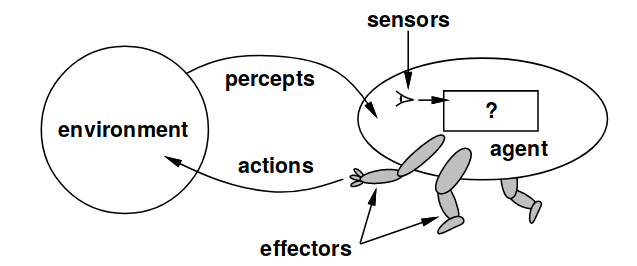
\includegraphics[width=0.5\textwidth]{russellnorvigagent.png}
	\caption{Russell and and Norvig's~\cite{russell2016artificial} agent}
	\label{fig:rnagent}
\end{figure}

\section{Kinship Theory}
\label{sec:kin}
Axelrod and Hamilton~\cite{evolution_of_cooperation} described the way in which cooperation in nature (with the exception of homo-sapiens) is almost always between related individuals. An earlier paper by Hamilton~\cite{kinhamilton} argues that individuals don't only work toward improving their own fitness, but towards what Hamilton defines as `inclusive fitness'. Inclusive fitness is the sum of a player's fitness and the fitness of each of their relations multiplied by a coefficient. The coefficient used by Hamilton is Wright's coefficient of relatedness, as illustrated in figure~\ref{fig:coefrelate}. It could be possible to create a similar coefficient of relatedness for use in a MAS.
\begin{figure}
	\center
	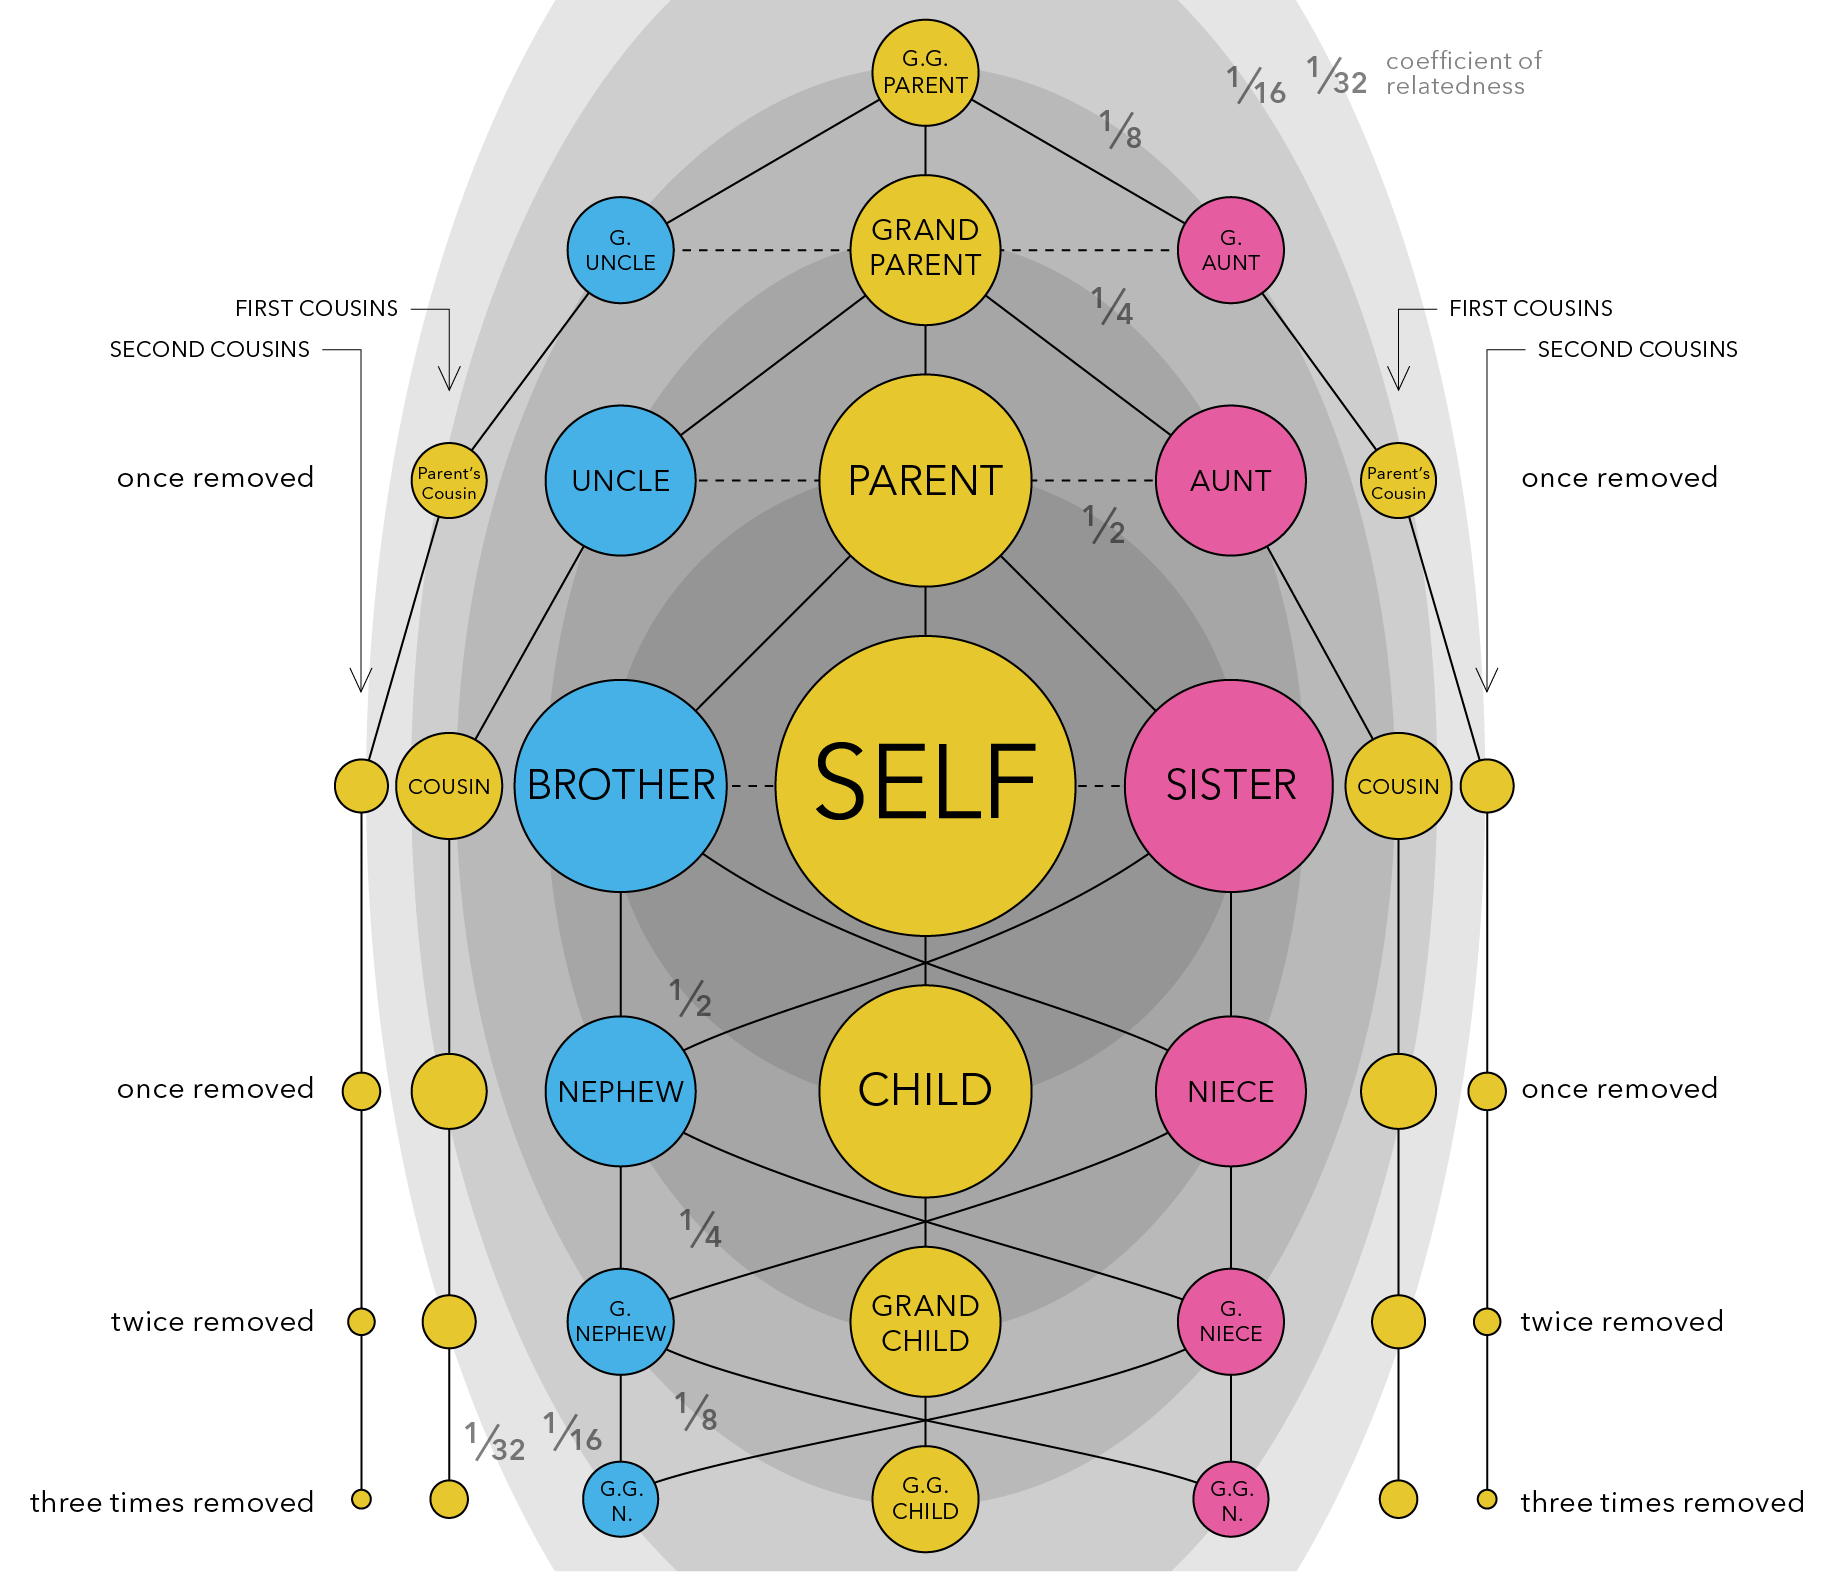
\includegraphics[width=0.5\textwidth]{coefrelate.png}
	\caption{Wright's coeffcient of relatedness by Citynoise - Own work, CC BY-SA 4.0, \url{https://commons.wikimedia.org/w/index.php?curid=37723128}}
	\label{fig:coefrelate}
\end{figure}
\par
Richard Dawkins~\cite{selfish_gene} advocated for the idea of the selfish gene. From a biological perspective, this idea postulates that actors are hardwired to propagate their genes. Dawkins asserts that this drive is due to the fact that genes are the true replicators evolutionarily rather than the actors themselves. Those with a high coefficient of relatedness to an individual are far more likely to carry their genes and to help them proliferate. This mechanism is similar to that presented by Hamilton~\cite{kinhamilton}, but with a biological backing. From a biological perspective this may make sense. However, it does not seem natural to translate an agent's strategy to the idea of genes.\par
Further, although it is possible to create a coefficient and an idea of relatedness similar to that of Hamilton's model~\cite{kinhamilton} for a MAS, it does not seem a natural translation. Another limitation to the use of kinship theory for MASs is that systems are ideally inclusive of individuals that can contribute to the society. For example, if an agent is looking to actively contribute to a society, but is not kin with the members, a MAS using kinship theory would exclude them and thus limit the abilities of that society.\par
Furthermore, Axelrod and Hamilton~\cite{evolution_of_cooperation} highlight that humanity is the exceptional society which does not limit itself to cooperating mostly only with kin. I would surmise that this exception is due to the higher level of intellect of homo-sapiens in comparison to other species. Many have suggested that the capabilities of AI could match or even surpass the intelligence of humans. Therefore, I would suggest that societies of IAs should also not be limited to the use of kinship theory to facilitate cooperation.\par
As such, I shall not be using kinship theory for my theoretical framework. I will be aiming to use a  mechanism that is inclusive of agents that aim to become valuable members of the society and also a mechanism which fits naturally into the agent's paradigm. 
\begin{figure}
	\center
	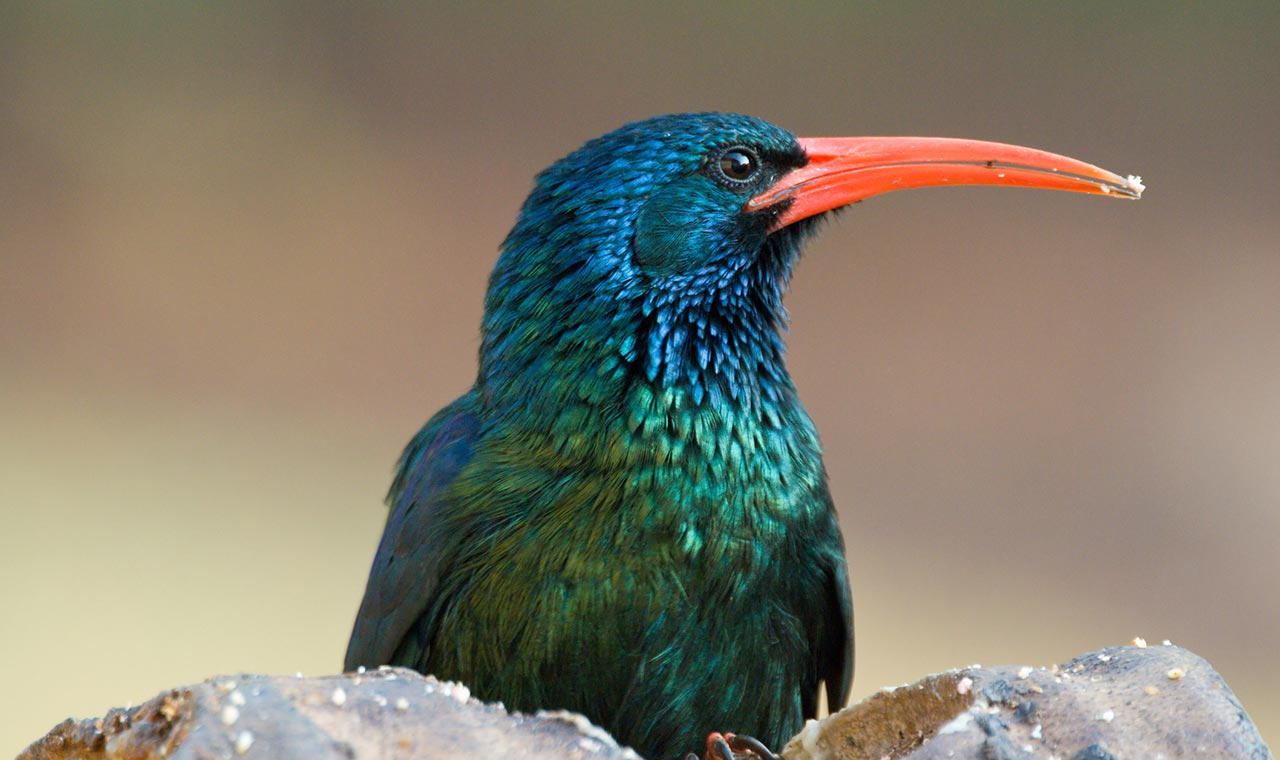
\includegraphics[width=0.5\textwidth]{green-wood-hoopoe.jpg}
	\caption{The Green Wood-Hoopoe native to Africa participates in cooperative breeding as the bird not only looks after its own chicks, but those of other breeding pairs~\cite{hoopoe}}
	\label{fig:hoopoe}
\end{figure}


\section{Reciprocal Altruism}
Reciprocal altruism is an idea most famously put forward by Robert L. Trivers~\cite{trivers1971evolution}. Trivers defines altruism as behaviour of one organism that benefits another to whom it is not closely related, while being apparently detrimental to the organism performing the behaviour. From this definition and from Trivers' description we can draw the meaning of reciprocal altruism to be altruism-based on the idea that the altruistic act will be returned.\par
This idea is a move away from limiting individuals to cooperating only with their kin and towards any individual that they believe their cooperation will be reciprocated by. Axelrod and Hamilton~\cite{evolution_of_cooperation} noted this concept as advantageous in explaining cooperation between unrelated individuals, such as is common between humans. I would argue that this concept is also more applicable to higher intelligence societies such as those possible from IAs.\par
In comparison to kinship theory, reciprocal altruism seems the more natural match to the agents paradigm as it does not require measures for relatedness between agents or conversion between an agent's strategy and the concept of a gene. These reasons make reciprocal altruism the more likely out of the two to apply to my problem.
\begin{figure}
	\center
	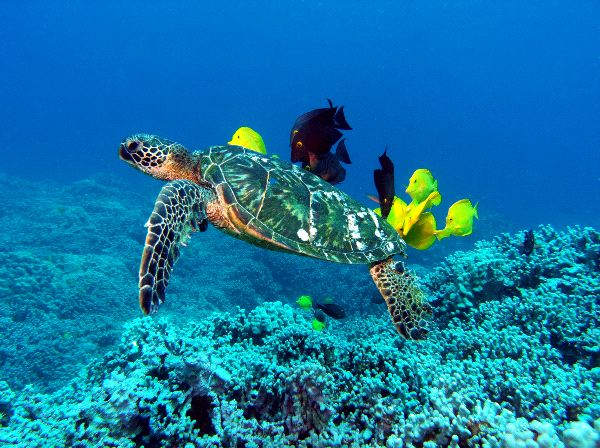
\includegraphics[width=0.5\textwidth]{Green_Sea_Turtle_Cleaning_Station.jpg}
	\caption{Cleaning symbioses such as that of the green sea turtle and surgeonfish including the yellow tang show that reciprocal altruism is possible between non-humans and even interspecies~\cite{turtle}}
	\label{fig:cleaning}
\end{figure}

\section{Axelrod, Hamilton and The Iterated Prisoner's\\ Dilemma}
\label{sec:ipd}
Axelrod and Hamilton~\cite{evolution_of_cooperation} also chose reciprocal altruism for further study over kinship theory. They recognised that kinship theory limits individuals to cooperation only with kin and at the time there had been more investigation into kinship theory. Of course the same cannot be said now, a there has been a lot of investigation into reciprocal altruism, mostly due to Axelrod and Hamilton~\cite{evolution_of_cooperation} and Trivers~\cite{trivers1971evolution}.
\begin{figure}
	\center
	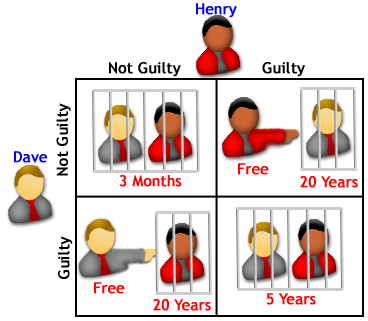
\includegraphics[width=0.4\textwidth]{LaymansIPD.png}
	\caption{A visualisation of the outcomes of the Prisoner's Dilemma~\cite{laymansipd}}
	\label{fig:ipdvis}
\end{figure}
\par
Game-theoretic modelling was used by Axelrod and Hamilton~\cite{evolution_of_cooperation} in their Iterated Prisoner's Dilemma tournaments. Imagine that a crime has been committed by two individuals who are now being interviewed by the police. Each individual can either choose to inform on the other, or stay loyal and say nothing.\par
Staying loyal is known as cooperating, informing is known as defecting. If an individual informs on the other they will receive no punishment, as long as the other has stayed loyal. However, if both defect they both receive a punishment. However, this punishment will not be as bad as for the individual who stays loyal when the other defects. This idea can be visualised in figure~\ref{fig:ipdvis}.\par
If this dilemma is not repeated, then a defector can get away with defecting and is not heavily punished. However, if the game is repeated in multiple rounds, then the mechanism of direct reciprocity comes into play. Direct reciprocity is a mechanism that works in the way that if I cooperate with you, you will hopefully cooperate with me in later rounds~\cite{five_rules_coop}.\par
Across multiple rounds during which when an individual does not know which round will be last, it may be more beneficial to cooperate, as following rounds will achieve a higher payoff if both cooperate than if both defect. This approach encourages cooperation without the need for pure altruism as it is a form of reciprocal altruism.\par
The focus of Axelrod and Hamilton's paper~\cite{evolution_of_cooperation} is to review the strategies of The Dilemma submitted to them by academics and teams working on the strategies throughout the world. Axelrod and Hamilton~\cite{evolution_of_cooperation} asked three questions of each strategy. Is it robust? Is it stable? Is it initially viable?\par
Robustness refers to the ability to thrive in an environment with a variety of strategies. Stability refers to the ability to - once fully established - resist invasion by mutant strategies. Initial viability refers to whether or not a strategy can establish itself in a non-cooperative environment.\par
Axelrod and Hamilton~\cite{evolution_of_cooperation} found two strategies with these three abilities: 'tit-for-tat' and 'all defect'. Nevertheless, later on, Nowak and Sigmund~\cite{nowak-1993a} found that 'Pavlov' ('win-stay, lose-shift') also has these abilities. The interesting part of 'Pavlov' and tit-for-tat is that they are nice strategies (they begin by cooperating) and that they also actively aid in the evolution of cooperation.\par
Another key aspect of The Iterated Prisoner's Dilemma is the way in which it has been formulated by Axelrod and Hamilton~\cite{evolution_of_cooperation}. In each round, players simultaneously either choose to cooperate or to defect, and the players earn points based on the outcome of the game as shown in the payoff matrix in table~\ref{tab:payoffmatrix}. Nowak~\cite{five_rules_coop} found that for the evolution of cooperation to occur, the cost-to-benefit ratio of the altruistic act must be less than the probability of another encounter for cooperation to evolve: $w>c/b$.\par
\begin{framed}
	\begin{center}
		\begin{tabular}{cc|c|c}
		& & \multicolumn{2}{c}{Player B}\\
		& & Cooperation & Defection\\
		\cline{1-4}
		\multirow{4}{*}{Player A} &\multirow{2}{*}{Cooperation} & A=3 & A=0\\
		& & B=3 & B=5\\
		\cline{2-4}
		& \multirow{2}{*}{Defection} & A=5 & A=1\\
		& & B=0 & A=1\\
		\end{tabular}
		\captionof{table}{The payoff matrix in a typical iterated prisoner's dilemma game (such as Axelrod and Hamilton's~\cite{evolution_of_cooperation}). A=x, B=y where x denotes the payoff for A and y denotes the payoff for B.}
		\label{tab:payoffmatrix}
	\end{center}	
\end{framed}
If the probability of subsequent encounters between two individuals is low, then it is very likely that cooperation will not evolve as there will be no sufficient reward. With the advent of huge networks spanning across the world and the drastic increase in devices across these networks, it is highly likely MASs will operate with IAs that are unlikely to re-meet.\par
This is a definite limitation to the use of direct reciprocity in MASs, and as such I do not see direct reciprocity as a strong contender to encourage cooperation on its own. One required property of a mechanism to encourage cooperation is that it must work when both re-meeting is unlikely and when it is likely. As such, direct reciprocity is not completely inadequate for the problem. However, it is insufficient when not combined with some encouragement for when chances of meeting again are low.\par
Extensive interest in reciprocal altruism in recent years has been focused towards direct reciprocity, including a number of available libraries such as the Axelrod Python library~\cite{axelrodproject}. I argue that to gain a better understanding of how we can work to facilitate cooperation between IAs,  we must look at a wider berth of options.

\section{Network Reciprocity}
Nowak - in his paper `The Five Rules of Cooperation'~\cite{five_rules_coop} - identified and compared five key mechanisms that can aid in the evolution of cooperation, two of which I have already discussed (direct reciprocity in section~\ref{sec:ipd} and kin selection in ~\ref{sec:kin}). The other three are network reciprocity (which I shall examine here), group selection and indirect reciprocity (both of which have their own sections).\par
Network reciprocity uses a graph of players and their connections. The players are represented by the nodes in the graph, with arcs representing connections between players. This idea ties closely to the networks that IAs may work across. Players with arcs between them interact with each other in rounds of The Prisoner's Dilemma. Nowak and May's~\cite{spatial} ealier work - which inspired Nowak's later paper~\cite{five_rules_coop} - did not give individual's any memory of past interaction.\par
This lack of memory limited Nowak and May to pure cooperators and pure defectors. In Nowak's book `Evolutionary Dynamics'~\cite{nowak2006evolutionary}, his exploration of evolutionary graph theory and spatial games (chapters 8 and 9) showed that the shapes of the lattice linking the players and different concentrations of cooperators and defectors on those shapes has a great effect on the evolution of cooperation. Visualised in figures~\ref{fig:coopinvdef} and ~\ref{fig:funnel}.\par
Nowak's~\cite{five_rules_coop, nowak2006evolutionary} and Nowak and May's~\cite{spatial} work on these games on graphs is limited in terms of strategies and also in terms of the fixed shape of its graphs. However, the work proves a key point: the structure of who interacts with whom can play a key role in supporting cooperation in large populations.\par
In real life, individuals will often mostly interact in their close social circles. For example, a Meerkat may interact with others of their family group, a drongo bird which calls to warn of predators, the predators and others who are geographically close to them. The graph in this case represents the close geographic ties.\par
I imagine the use of Nowak~\cite{five_rules_coop, nowak2006evolutionary} and Nowak and May's~\cite{spatial} work to employ a network not as a representation of a physical network structure or geography, but as a representation of the choices made by IAs with whom they wish to interact with.\par
This network would be a constantly changing and adapting network of IAs. The IAs would not concern themselves with the strategy they employ towards whom they are forced to interact with. Instead, their strategy is to select those whom they wish to interact with, thus, effectively constructing a graph of network reciprocation. How these changing graph connections would affect cooperation is unbeknownst to me. Indeed, whether Nowak's rules would still apply would be interesting to find out.\par
Nowak~\cite{nowak2006evolutionary} found that some shapes supported cooperators in groups. Cooperators could make use of these shapes by deliberately forming them to protect one another. While another set of shapes were found as `amplifiers' for evolution, maybe defectors could make use of these sorts of shapes to invade groups of cooperators.\par
I can see IAs having strategies as to how to build these shapes. However, an issue may arise in which cooperative agents find it hard to reach out to other cooperators which are not part of their current shape.As such, there may be possible prevention of the spread of cooperation, thus limiting these groups. However, this concept is worth investigating, and the problem could possibly be overcome using some kind of bridging mechanism.\textcolor{red}{Compare to \cite{jennings2000agent} organisational relationships}.
\begin{framed}
	\begin{center}
		\begin{tabular}{c|cc}
		& \textcolor{blue}{A} & \textcolor{red}{B}\\	
		\hline
		\textcolor{blue}{A} & a & b\\
		\textcolor{red}{B} & c & d\\
		\end{tabular}
		\captionof{table}{The payoff matrix for when individuals interact. Cooperators are in blue and are called A, and defectors in red and called B. Taken from Nowak's book Evolutionary Dynamics~\cite{nowak2006evolutionary}.}
		\label{tab:networkmatrix}
	\end{center}	
\end{framed}
\begin{figure}
	\center
	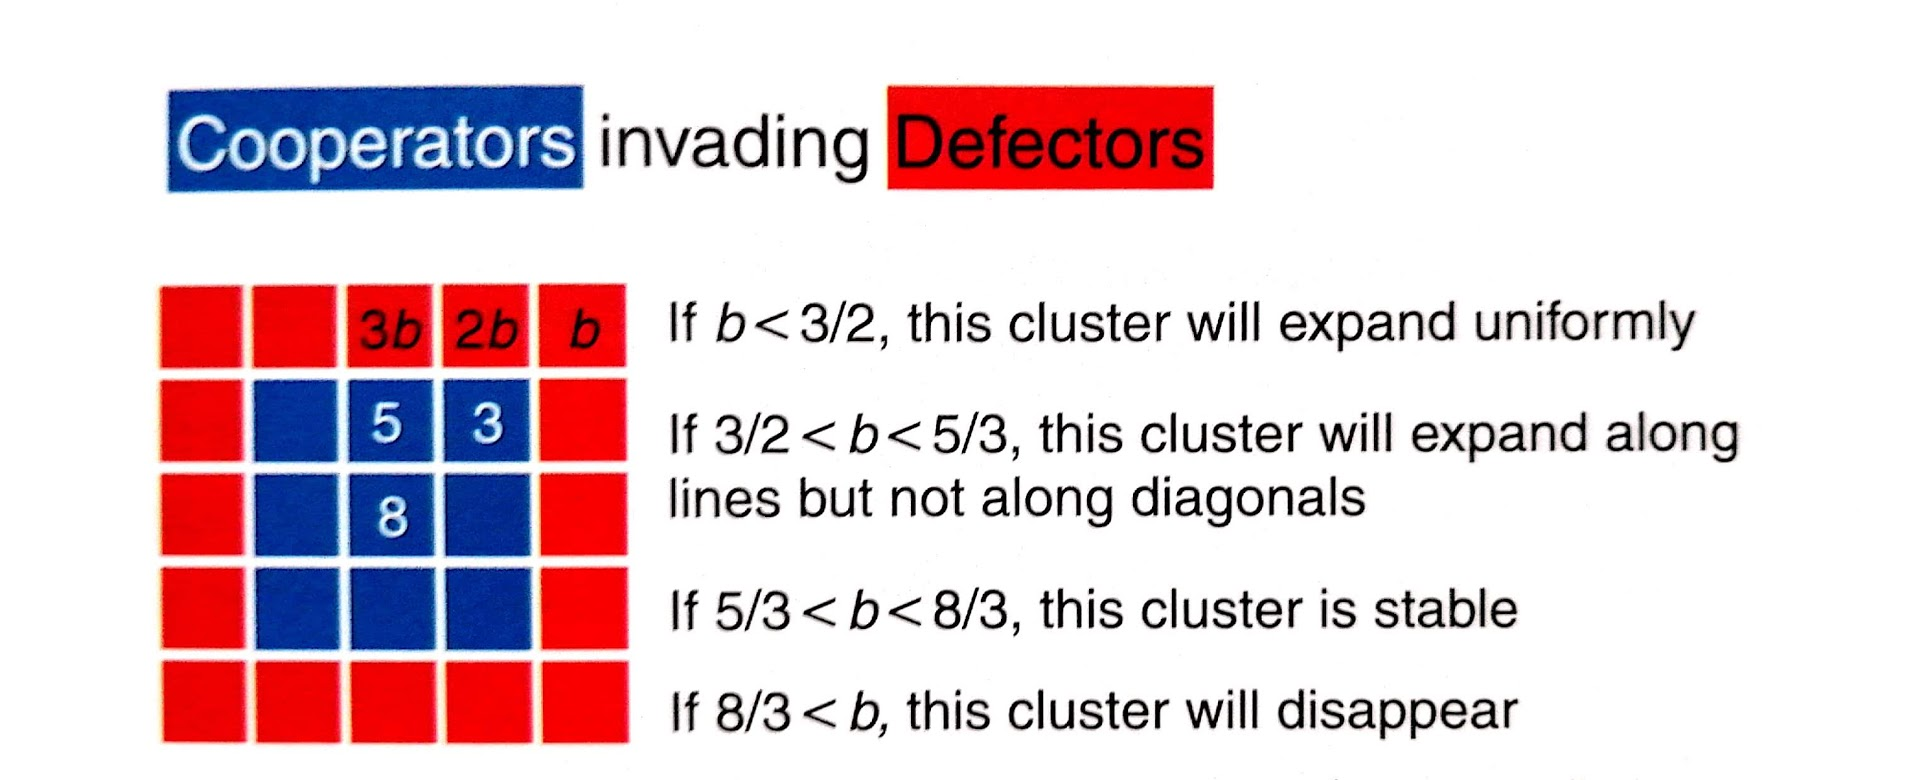
\includegraphics[width=0.5\textwidth]{cooperators-invading-defectors.jpg}
	\caption{How can cooperators invade defectors? Taken from Nowak's book Evolutionary Dynamics~\cite{nowak2006evolutionary}. The squares represent nodes and the players interact with the players to each side of them and diagonally. The value b is from the payoff matrix in table~\ref{tab:networkmatrix}}
	\label{fig:coopinvdef}
\end{figure}
\begin{figure}
	\center
	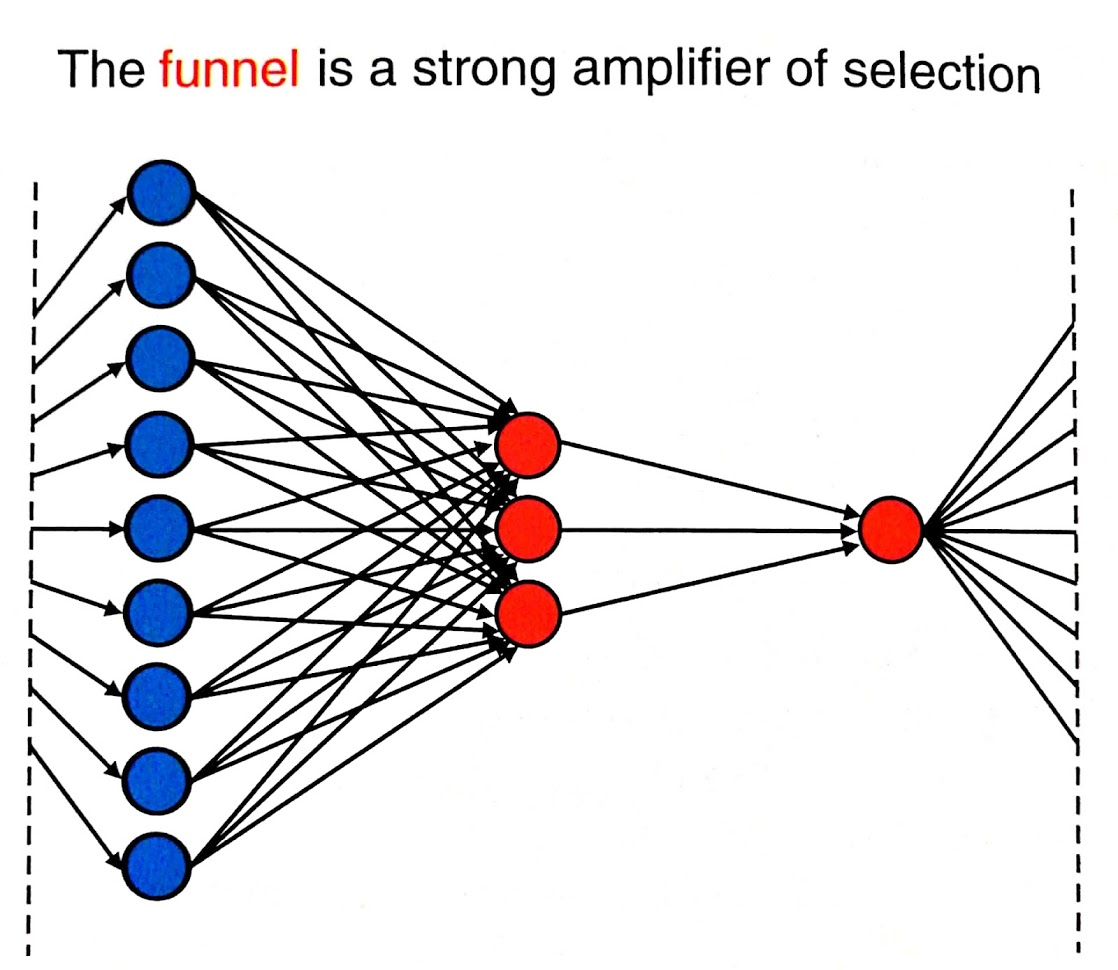
\includegraphics[width=0.5\textwidth]{funnel_amplifier.jpg}
	\caption{Shapes that can amplify selection include the funnel, the star and the superstar~\cite{nowak2006evolutionary}}
	\label{fig:funnel}
\end{figure}


\section{Group Selection}
Group selection is another mechanism described by Nowak~\cite{five_rules_coop}. This mechanism splits one population into multiple groups. Within these groups, The Prisoner's Dilemma is played and reproduction occurs which is proportional to each players payoff. If using the payoff matrix in table~\ref{tab:payoffmatrix}, then cooperators can work together to produce a payoff of three, while defectors can only produce five or two for both players in the interaction.\par
The group size increases until a certain point, at which the group may split. If the group does split (which is stochastically chosen) then another group is destroyed. The effect is multi-level selection.\par
Nowak found that due to the higher payoff between cooperators, reproduction will occur more quickly within the groups they dominate, than the groups filled with defectors. The faster the reproduction, the quicker the group size grows, making it more likely for groups of cooperators to survive while groups of defectors will shrink and be destroyed. These dynamics are displayed in figure~\ref{fig:group}.\par
Traulsen and Nowak~\cite{multilevel_nowak} limited themselves to cooperators and defectors, but noted that other strategies could be built into their model. A limitation to applying group selection to MASs is the groups themselves. In this model, individuals do not interact with individuals in other groups, creating a barrier between them.\par
Even our current networks span the globe and don't always have harsh barriers between them - even when security is high, these barriers can often be broken. Furthermore, IAs are often built to be of service to others and limiting them to being of service only to one group greatly reduces the service an agent can supply and limits the society as a whole . Finally, the group mechanics of splitting and destroying another group of individuals does not naturally match the paradigm of MASs.\par
I would suggest that this is not a mechanism which would be useful to apply to MASs unless you are modelling clusters of agents, with each cluster in competition. This idea is not the aim of my project; however it could be another interesting project to take up.
\begin{figure}
	\center
	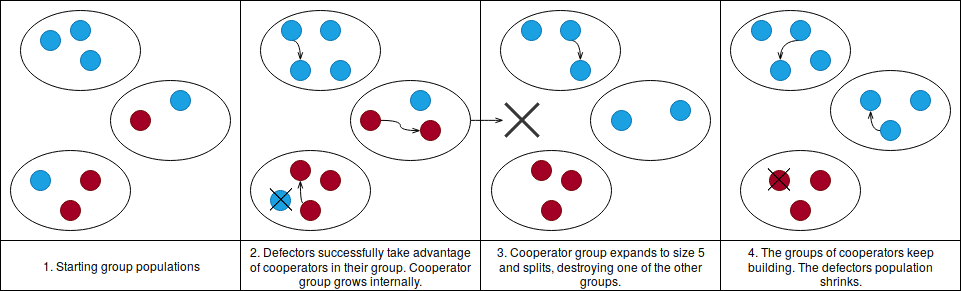
\includegraphics[width=\textwidth]{GroupSelection.png}
	\caption{The dynamics of multi-level selection as described by Traulsen and Nowak~\cite{multilevel_nowak}.}
	\label{fig:group}
\end{figure}

\section{Indirect Reciprocity}
The final mechanism I will be discussing from Nowak's Five Rules of Cooperation~\cite{five_rules_coop} is indirect reciprocity. This concept is promising for use in MASs as it solves the failure of direct reciprocity's failure with regard to when re-meeting is low. In a large society or a vast network in which agents are likely to operate in success when re-meeting is low is an important property. We will see later on that the two mechanisms can be combined.\par
Indirect reciprocity uses the group mechanic of reputation to encourage cooperation. Alexander~\cite{alexander1987biology}, who was an early advocate the idea, focused on human reciprocal altruism, however, subsequent research has abstracted away from the biology~\cite{phelps_game_theoretic_analysis, imagevsstanding, evol_indirect_image, evoldirindir, five_rules_coop, leimarhammer, sugden2004economics, gossip_alt, mui2002computational}. The idea is that if an individual cooperates with another individual, then their reputation will be enhanced in the community. This boost of reputation makes it more likely that they will be helped by others later on. Thus this mechanism a form of reciprocal altruism.\par
According to Nowak and Sigmund~\cite{evol_indirect_image} the reputation mechanic requires a higher level of intelligence than direct reciprocity, due to the complexity of group mechanics in the system. It is this kind of higher level intelligence which is required to reason about events in a group that could be a key part in the development of IAs.\par
Due to this reason, I feel that either indirect reciprocity or possibly a combination of both direct and indirect reciprocity is a good candidate for a mechanism to study further. For the rest of this literature review I will consider both past approaches to indirect reciprocity and other factors in the mechanism that can be used to facilitate the evolution of cooperation.
\begin{figure}
	\center
	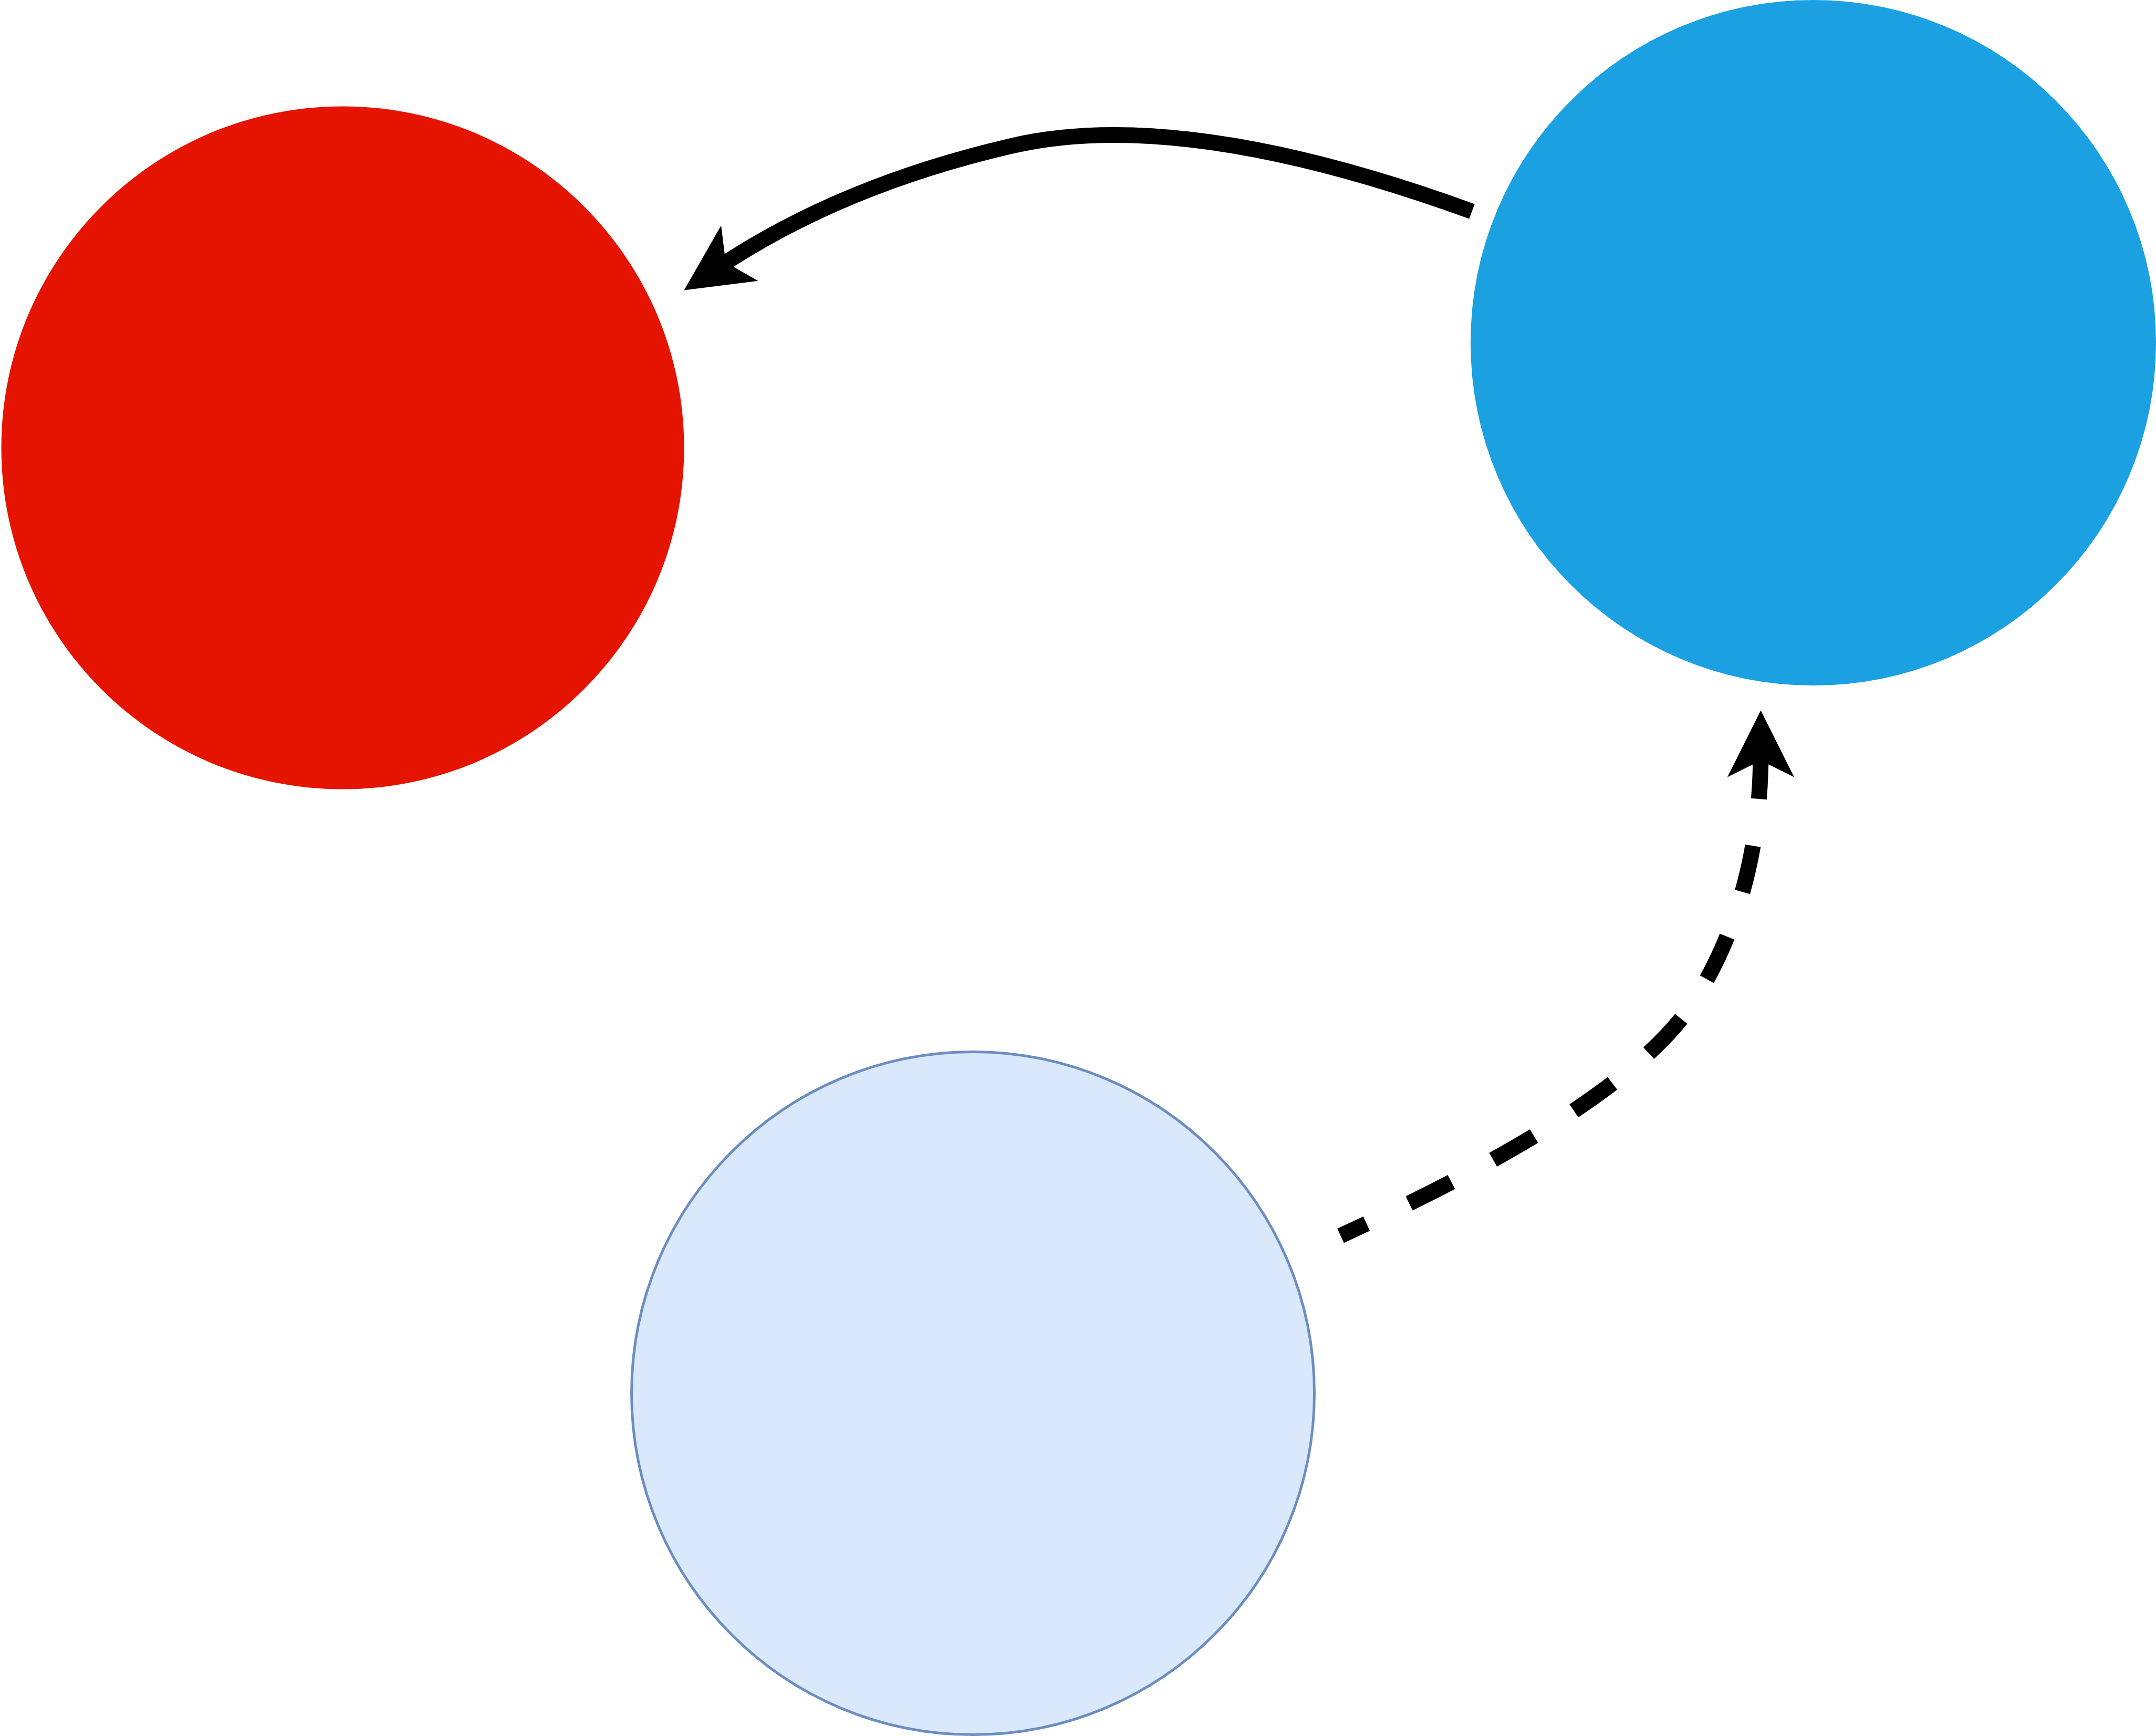
\includegraphics[width=0.5\textwidth]{IndirectRec.png}
	\caption{The main idea of indirect reciprocity from Nowak~\cite{five_rules_coop}}
	\label{fig:indir_rec}
\end{figure}

\section{Nowak and Sigmund}
\label{sec:nowak_sig}
According to Gilbert Roberts~\cite{evoldirindir}, Nowak and Sigmund~\cite{evol_indirect_image} is the most influential model on indirect reciprocity. Therefore, I shall examine this model of indirect reciprocity first. Nowak and Sigmund begin by stipulating that human cooperation is due to people's `image' of each other, which is comparable to reputation. Nowak and Sigmund converted the image to an integer score between -5 and 5 for simplicity.\par
The idea is simple, cooperation increases your image score by 1 and defection reduces it by 1. The higher your image score the more likely it is you will receive help. Nowak and Sigmund claim that this mechanism channels cooperation toward valuable members of the society of players.\par
Nowak and Sigmund note that the use of image scores and indirect reciprocity itself, leave a system open to anticipation, planning, deception and manipulation. These 4 concepts seem closely related to possible happenings in MASs. Deception and manipulation are two factors that I think are worth experimenting with. At the same time, anticipation and planning are a key part of agent design in multiple languages and frameworks. To highlight this point it was such an important drawback of the Agent0 language~\cite{shoham1991agent0}, Becky Thomas created a new language - PLACA~\cite{thomas1993placa} - which allowed agents to plan, among other improvements.\par
The framework created by Nowak and Sigmund is simplified from Alexander's~\cite{alexander1987biology} idea of human reciprocal altruism. Nowak and Sigmund describe a framework in which there is a population of individuals which act as a pool to select pairs in which one player is the donor - who can choose whether to cooperate or defect - and the other is the recipient of this action. A cooperation costs the donor $c$ to its fitness and benefits the recipient's fitness the value of $b$ where $b>c$. Whereas a defection costs nothing and the recipient is not benefitted. This is shown in the payoff matrix in table~\ref{tab:indirrec_payoffmatrix}.\par
\begin{framed}
	\begin{center}
		\begin{tabular}{c|c|c}
		\multirow{2}{*}{Donor Action} & \multicolumn{2}{c}{Payoffs}\\	
		& Donor & Recipient\\
		\hline
		Cooperation & -1 & 2\\
		\hline
		Defection & 0 & 0\\
		\end{tabular}
		\captionof{table}{The payoff for Nowak and Sigmund's~\cite{evolution_of_cooperation} indirect reciprocity model}
		\label{tab:indirrec_payoffmatrix}
	\end{center}	
\end{framed}
As noted above, these actions also affect the donor's image score, but Nowak and Sigmund add a caveat when using the idea of onlookers. A specified size group is randomly selected from the population to view an interaction, limiting the spread of reputation information. This concept is displayed graphically in figure~\ref{fig:onlookers}. The concept of onlookers was added due to the realisation of Nowak and Sigmund's that in a group that is spread over a wide geographical area, not all individuals will be able to view each interaction. This sparse nature of interactions is of course especially likely in MASs. Image scores now become one player's view of another rather than a community view of the player. A matrix $ImageScore$ is used to store these scores.\par
The discriminator is the strategy of choice for Nowak and Sigmund. This strategy stores a number $k$, and when the individual $u$ using that strategy is a donor to the individual $v$, $u$ cooperates if the value $ImageScore[u,v]>=k$ otherwise it defects. This strategy is incredibly simple yet effective, and is displayed graphically in figure~\ref{fig:image_discriminator}. The model also includes the defector and cooperator strategies. Nowak and Sigmund detailed more strategies. These strategies base their decisions not only on that of the recipient's image score but also their own. In this way, the individual will be able to decide whether it is important to boost their reputation in the system in order to receive cooperation or not.\par
Nowak and Sigmund hypothesize and give evidence supporting the idea that the length of the generation is important to the evolution of cooperation. They highlight that when $m$ donor-recipient pairs are selected in succession in a population of size $n$, a player is likely to be selected as part of a pair $2m/n$ times. According to their evidence, the higher this value of $2m/n$, the more likely cooperation will evolve.\par
As previously noted Herbert Spencer coined the phrase ``Survival of the fittest''~\cite{spencer1864principles}. This principle is put to work by Nowak and Sigmund in their reproduction mechanism. The higher the fitness of an individual the more likely it is that they will reproduce into the next generation. They also include a chance for random mutation in  reproduction.\par
Another idea put forward and evidenced by Nowak and Sigmund is that the evolution of cooperation is dependent upon the donor's knowledge of the image score of the recipient. This chance of knowing an image score is limited by the concept of onlookers. However, in Nowak's 2005 paper on the five rules of cooperation~\cite{five_rules_coop} he talks about using `gossip' as an alternative to direct observation. Gossip and social ability are interesting concepts in MASs. According to Wooldridge and Jennings~\cite{wooldridge_jennings_1995}, social ability is a key property in even a weak notion agents.\par
Nowak and Sigmund stress that discriminators are not 'tit-for-tat' players as used in direct reciprocity, because they use the experience of others. However, the similarity lies in the way that discriminators punish those with lower image scores due to their uncooperative actions, but are forgiving to those who improve and cooperative to those who they consider 'good'. This strategy can also be considered `nice' if it is using a value of $k<=1$ as it will cooperate even when the recipient has no past action history.\par
The model laid out by Nowak and Sigmund is succinct and a good basis for looking at interactions in multi-agent systems. However, there are limitations to their approach in the context of MASs. The first limitation I will highlight is the way in which reputation is implemented. In the version without onlookers each player has a global image score and even in the version with onlookers there is a public matrix encoding all image scores.\par
Image scores could be seen as a community view of an individual. However, I argue that the idea that image scores are attempting to capture (reputation) is actually more personal. Although there might be a rough consensus as to an individual's general reputation among people in a society, this reputation is often conveyed through social means and is subject to the personal interpretation of each individual.\par
According to Russell and Norvig~\cite{russell2016artificial}, IAs use an internal state. In the BDI model~\cite{rao1995bdi} the internal state is the beliefs of an agent. It is in this internal state or a belief-system, I argue, that image scores should be stored in order for an agent to have full control over them. Multiple trust models could be devised to manage these image scores. This idea is a closer match to the agent paradigm and it would allow for a truly distributed system.\par
Indirect reciprocity makes a good candidate for use in MASs and this model is both very influential and a good basis for those MASs. The model includes extensive interesting aspects that have been examined carefully including the onlookers and reproduction mechanisms, and also includes ideas that have not been fully researched such as a gossip systems and using deception and manipulation to affect the system. These features allow more room for me to explore if I use Nowak and Sigmund's model as a basis, with a few alterations to more closely match the MAS paradigm.
\begin{figure}
	\center
	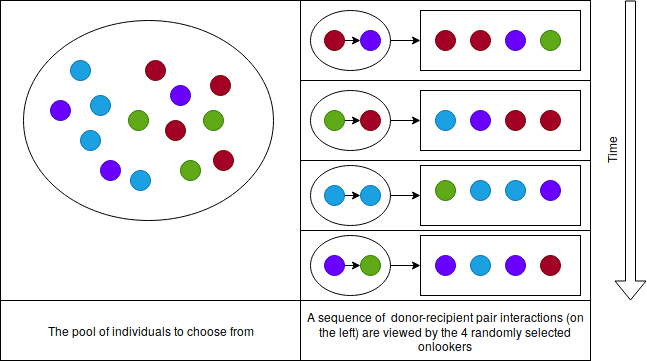
\includegraphics[width=0.7\textwidth]{Onlookers.png}
	\caption{The selection of a sequence of donor-recipient pairs and onlookers in Nowak and Sigmund's~\cite{evol_indirect_image} model of indirect reciprocity. The macro-view of indirect reciprocity. The lines and arrows show the spread of information.}
	\label{fig:onlookers}
\end{figure}
\begin{figure}
	\center
	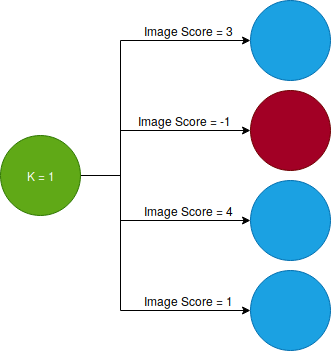
\includegraphics[width=0.3\textwidth]{Image_Scoring.png}
	\caption{On the left an image scoring discriminator with K=1. On the right the agents the discriminator is a donor for. Blue agents represent where there would be a cooperation from the donor, red represents when the discriminator would defect against them. The rule is when $Image Score >= K$ cooperate else defect.}
	\label{fig:image_discriminator}
\end{figure}

\section{The Standing Strategy and Further Limitations of Nowak and Sigmund}
Leimar and Hammerstein~\cite{leimarhammer} criticised Nowak and Sigmund's~\cite{evol_indirect_image} limited range of strategies. They also highlighted the abilities of another strategy, the standing strategy, over image scores.  The standing strategy was first described by Sugden~\cite{sugden2004economics} and and uses a `switch'~\cite{evol_indirect_image}.\par
Milinski \textit{et. al}~\cite{imagevsstanding} described the standing strategy as the idea that an individual does not only aim for a good fitness but also a good standing. Each individual holds other individuals in either a good or bad standing, which starts out as good until perceived otherwise. The event that causes the switch from good to bad is an individual defecting against another with a perceived good standing.\par
The idea is that it is morally incorrect to defect against a good individual, but defecting against a bad individual is acceptable as it punishes those members of society that are not valuable. There is conflict between the use of image scores and the standing strategy.\par
The argument for the standing strategy is as follows: When using image scoring, if a discriminator has $k=0$ and is a donor to another with an image score of $-1$, they will defect. This action is seen as punishing a bad individual, as it channels fitness away from bad members of the society. However, the donor's image score is reduced by 1. This change in score decreases the chance that the donor will receive cooperation from others, so there is no real incentive for them to punish the bad members of that society, except for pure altruism.\par
Conversely, the standing strategy only reduces the reputation of those who defect against good individuals. Therefore, punishing bad members of the society has no negative effect on those members. Leimar and Hammerstein~\cite{leimarhammer} argue that Sugden's version of indirect reciprocity and his use of the standing strategy are more robust than Nowak and Sigmund's image scoring.\par
Milinski \textit{et. al}~\cite{imagevsstanding} analysed Leimar and Hammerstein's argument, suggesting that they were correct under conditions which allowed for perfect perception of events and unlimited memory capacity. However these conditions are not always true, especially in a MAS in which the environment is inaccessible~\cite{russell2016artificial}.\par
Nowak and Sigmund claimed that indirect reciprocity is open to deception and manipulation, especially when we consider the use of gossip in a system. Gossip opens IAs to imperfect perception of other IAs. Therefore, it would be interesting to see which strategy is more effective in a system in which other IAs actively attempt to deceive using gossip, and the information received is not always perfect.

\section{Mixed Reciprocity Models}
Roberts~\cite{evoldirindir} and Phelps~\cite{phelps_game_theoretic_analysis} noted that indirect reciprocity is focused towards interactions with other individuals with whom the donor has no previous interactions. However, what about when re-meeting is more likely? I stipulate that an individual is affected by both being the recipient of actions and their observation of actions. Roberts engaged with the issue by introducing an experience score. This experience score works similarly to an image score but is bounded by -1 and 1. It increases when the individual is a recipient of a cooperation, and decreases when receiving a defection.\par
Roberts also created a version of the standing strategy which uses an image score (-1 to 1). However herein, the value changes according to the rules of the standing strategy rather than Nowak and Sigmund's rules.\par
Both Roberts and Phelps measured the use of indirect reciprocity against the use of direct reciprocity. Roberts concludes that indirect reciprocity is the more popular decision mode under conditions in which re-meeting was less common, and direct was more popular when re-meeting was frequent. On the other hand, Phelps' experiments garnered different results being that in small groups direct and indirect reciprocity exist in equilibrium.\par
Similarly to Nowak and Sigmund~\cite{evol_indirect_image}, Roberts I believe falls short in recognising how personal interpretation of events are. There are many different trust models a player could use by mixing interpretation of events in which they are the recipient and also in which they are not the recipient. For example, it could be expected that being on the receiving end of a defection means that a player is likely to be more hardline, than when they observe a defection against another. However, Roberts limits the study to using a simple experience score.\par
I would suggest using a model similar to that I described in section~\ref{sec:nowak_sig}, in which interpretation of events is up to an agents trust model. Some trust models could interpret events when the agent is the recipient different to those in which they are observing.

\section{Gossip}
Nowak and Sigmund~\cite{evol_indirect_image} realised the issues surrounding the fact that all individuals being able to view interactions in their simulation framework is not concomitant with real life. As such, they introduced the idea of onlookers as noted in section~\ref{sec:nowak_sig}. An issue with limiting observation is that knowing an accurate image score of a player is important to the evolution of cooperation in an indirect reciprocity system. Nowak~\cite{five_rules_coop} suggested using gossip to spread information regarding image scores in their simulation framework.\par
Sommerfeld \textit{et al.}~\cite{gossip_alt} conducted an empirical study on gossip between cooperative and uncooperative individuals in an indirect reciprocity setup. The experiment consisted of humans playing a number of indirect reciprocity rounds to build up a cooperation history, and then a smaller number of gossip rounds. These rounds were then repeated to see how the individuals reacted to the gossip.\par
The focus of the experiment was to look at gossip composition, gossip transfer and resulting behaviour. The findings included that gossip is an effective method of spreading reputation information in an indirect reciprocity system, on fulfilment of some conditions, the first of which is the truthfulness of the gossip. Gossip must accurately reflect the behaviour of the subject of the gossip.\par
Another condition is the comprehensibility of the gossip. The language used in the gossip must be interpretable by the recipient of the gossip. In an agent system this condition would require an agent communication language (ACL) (such as KQML~\cite{finin1994kqml} or FIPA-ACL~\cite{o1998fipa}) and would also require the content of the messages that use this language to be interpretable by the recipient agent. The final condition is that individuals must act accordingly based on the gossip they receive.\par
These three conditions of a system would have to be created by building strategies for agents that attempt to uphold them, and a communication language to support accurate and interpretable information. Nowak and Sigmund~\cite{evol_indirect_image} identified that indirect reciprocity systems can be effected by deception and manipulation from malicious players. The addition of gossip creates a meta-game on top of the indirect reciprocity system. Players must have a trust model that differentiates between dealing with gossip and with directly observed interactions, and a strategy on spreading gossip effectively.
\begin{figure}
	\center
	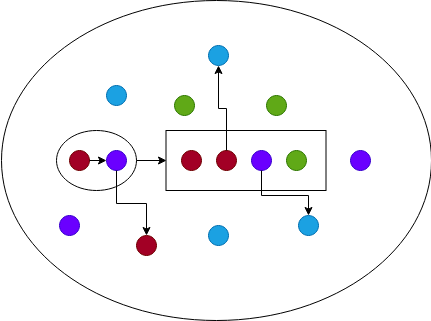
\includegraphics[width=0.5\textwidth]{Gossip_and_onlookers.png}
	\caption{The spread of information (shown through the lines) through a population using indirect reciprocity with gossip and onlookers}
	\label{fig:gossip_and_onlookers}
\end{figure}

\section{Mui's Computational Models of Trust and Reputation}
Mui~\cite{mui2002computational} presented an indirect reciprocity simulation framework similar to Nowak and Sigmund~\cite{evol_indirect_image} that spreads social information through `acquaintance networks' to inform a donor's decision. An individual in this framework builds up a network of players whom they meet through interaction, their `acquaintance network'. If this individual is then a donor in a donor-recipient pairing the individual consults their acquaintance network regarding the recipient. The information gathered from this network helps a donor to decide if they can trust the recipient to reciprocate their cooperation; known as `collective memory'.\par
Baumeister \textit{et al.}~\cite{baumeister2004gossip} advocated for the idea that gossip is used for four functions, including strengthening bonds between the gossiper and recipient, enabling the spread of information about the subject (one function for each positive and negative reasons), and helping to educate individuals about the complex cultural systems they reside in.\par
I would argue that indirect reciprocity systems and MASs are complex cultural systems in which gossip can be applied for these four functions. Mui's acquaintance networks support this gossip functionality to a certain extent; however they are limited by the lack of proactivity of gossip. Sommerfeld \textit{et al.}~\cite{gossip_alt} highlighted the willingness of their participants to spread gossip, and the last function of gossip proposed by Baumeister \textit{et al.}~\cite{baumeister2004gossip} (cultural education) suggests that for gossip to be most effective the gossip should be proactively spread.\par
As a result, I believe that a theoretical framework which uses gossip should allow a proactive social ability  by using gossip as an action at times at which an agent is not acting as a donor. 

\section{Summary}
From the information I have laid out in the previous sections in this chapter I have become aware of a number of options which could be used to facilitate the evolution of cooperation in MASs. I hold the two most pertinent options to be network reciprocity and a combination of indirect and direct reciprocity.\par
Using network reciprocity in which agents choose with whom they wish interact with, forming social networks and circles would be extremely interesting. It would also be an informative simulation of agents working across a network, selecting which other agents with whom they wish to interact to solve problems and complete tasks.\par
However these agents may have to work with others whom they have no experience with. Indirect reciprocity seems an ideal mechanism for helping decide on these issues. As such, I will be researching further into the trust models and the effects of indirect reciprocity on the evolution of cooperation that indirect reciprocity has.\par
My model will be inspired by that of Nowak and Sigmund's~\cite{evol_indirect_image} influential model. I will be using concepts including onlookers, reproduction based on fitness scores and sequential selection of donor-recipient pairs from a pool of players. However I will also be looking at how gossip, deception and manipulation affect the system.\par
In some systems re-meeting will be likely, especially in the close circles I anticipate a network reciprocity system would have. As such, I will be looking at using a mixed reciprocity model, in which I will not be implementing any image score matrix into the system, but will allow agents to hold their interpretation of other agents in their internal state.\par
Agents will be able to use multiple different strategies. These strategies will include the standing strategy~\cite{sugden2004economics} and Nowak and Sigmund's discriminator~\cite{evol_indirect_image}. It will be interesting to see which performs better within situations in which the spread of information can be imperfect.\par
Strategies will have different trust models which can interpret both information from when the agent is a recipient of an action, direct observation of other's actions and from gossip received which conveys reputation information. It will be important to find trust models that can deal well with deception, whilst still being open enough to allow trustworthy gossip to affect their decisions. A key aspect of study for me will be social ability and the effect of gossip and the interpretation of gossip on the evolution of cooperation. The system I devise will use gossip proactively.\par
As highlight by Leimar and Hammerstein it is also important to differentiate between uncooperative actions to bad and to good agents. As such a good trust model may act more harshly against those who are uncooperative when they are the recipient, as they can guarantee themselves as having good intentions.\par 
A subsequent project or study could use the version of network reciprocity which I have described. The model of the new study could use the trust models and information about them revealed from this to deal with handling players that have not been met before. Furthermore, this new study could also use the information revealed regarding use of social ability to spread reputation information.

\chapter{Framework}
\textcolor{red}{Excellent understanding and insight. Conceptual framework underpins study. Comprehensive expert account of topic. Well thought through Software Engineering content.}
\section{Introduction}
\textcolor{red}{Relate to background.\\
Objective 4.\\
Look at summary of Lit review + end of each section of lit review}

\section{Theoretical}
\subsection{Introduction}
In the previous chapter I explored possible mechanisms and ideas that can be used in multi-agent systems to study interactions between agents and to facilitate the evolution of cooperation between agents. This led me to a decision that I will use a mixed reciprocity inspired mainly by Nowak and Sigmunds~\cite{evol_indirect_image} model with elements from many of the sources I used. In this section I will be using these elements, ideas and mechanisms to formulate a theoretical framework for my multi-agent system to use.\par
This section is focused on objective four from my aims and objectives section~\ref{sec:aao} and includes the environment, percepts, actions, an agent communication language and gossip model, a reproduction and fitness scoring mechanism, an agent architecture, and agent strategies and trust models.

\subsection{Environment}
\label{subs:env}
There are many different definitions of agency~\cite{franklin1996agent}. Russell and Norvig~\cite{russell2016artificial} gave a wide ranging definition of an agent as being situated in an environment, which the agent can perceive through various sensors and act in using actuators. Their notion of an agent is visually described in figure~\ref{fig:rnagent}. Wooldridge~\cite{wooldridge2009introduction} describes an agent as able to work out the actions required to meet it's design objectives.\par
These two different definitions cover the two aspects of an agent: the physical and the mental. An agent's design objectives will work within the bounds of an environment, so before we discuss any agents in this system I will discuss the environment it shall be working in.\par
An instance of the environment in my system will be known as a community. A community contains a number of generations, which each contain a set of agents. These sets of agents will act as a pool to select donor-recipient pairs and onlookers for those pairs from.\par
The environment has distinct timepoints, which varies depending on how the number and length of generations variables are set. Say these range from $1..n$ and there are generations $1..k$ where $k<n$ and $n\%k=0$. The generations occur in an order, and the range of timepoints are distributed evenly across each generation like this:\par \centerline{$\{1..(n/k),\ (n/k+1)..(2n/k),\ ..,\ (n-(n/k)+1)..n\}$}
\par
The environment will work using a perceive-decide-execute cycle, much like Russell and Norvig's~\cite{russell2016artificial} episodes. Each step of the cycle is a timepoint. Agents will receive perceptions at the start of each cycle step, these may come from the environment themself or from the actions of agents the previous cycle step. The steps are synchronised, this prevents actions from a timepoint affecting other agents decisions at the same timepoint. Synchronicity keeps the environment static for the period in which an agent is deciding.\par
In each timepoint there is exactly one donor-recipient pair and for that pair there is a group of onlookers randomly selected from the rest of the generations pool of players. The onlookers and recipient receive a percept in the next cycle step of what they observed/received in that interaction.\par
Percepts (discussed in subsection~\ref{subs:percepts}) are sent to agents at the beginning of each cycle step, the agents will then be asked to decide on an action (subsection~\ref{subs:actions}) and these actions shall then be executed (subsection~\ref{subs:execution}) in the system.\par
As discussed each generation contains a set of players which participate in the cycle steps for each timepoint of that generation. But how are these sets of players selected? For the first generation a number of agents and associate strategies (subsection~\ref{subs:strat}) with them.\par
One of the aims of this project is to discover successful agent strategies for the mixed reciprocity model. An optimisation problem is where we have a set of solutions (strategies) and want to find the most effective one~\cite{optimisation_problems}. Francq~\cite{optimisation_problems} puts forward that genetic algorithms (a type of meta-heuristic) are superior to most traditional heuristics. Natural selection is the basis for genetic algorithms and contains 5 steps: reproduction, crossover, mutation, inversion and evaluation. Due to the nature of agents, we are only specifically interested in reproduction and mutation.\par 
Just like in The Iterated Prisoner's Dilemma I will use a genetic algorithm (GA) to discover the most effective solution for the given parameters~\cite{mitchell1998introduction}. How my system will work as a GA is outline in subsection~\ref{subs:reproduction}.\par
Russell and Norvig outline 5 different properties. I conclude that the environment I have delineated have the following properties.\par
Inaccessibility or partial observability, as the sensors of an agent cannot detect all aspects relevant to an action choice. They cannot know the intentions of other agents, which is key to deciding on whether an agent should cooperate or not. Agents can also not view all interactions, to inform their decisions, using the onlookers mechanic. However, lots about the environment will be observable. For example, agents will not need to `discover' each other they will have knowledge of all other agents in the generation.\par
I also argue that the system is deterministic from a generational point of view. Milinski \textit{et al.}~\cite{imagevsstanding} claimed that individuals using the standing strategy aim for a good standing, and Leimar and Hammerstein~\cite{leimarhammer} argue that the standing strategy is good as it allows individuals to punish bad individuals. However take 3 agents a, b, c and d. Agent b has defected previously against d who has a good standing according to a. Agent a then chooses to punish b but is still believing this won't reduce their standing. However, agent c did not observe b's defection against d but is an onlooker for c's defection against b.\par
From the proceedings the environment appears to be non-deterministic, as there is more than one outcome to an action. However, this is due to the partial observability of the environment not the determinism, as highlighted is possible by Russell and Norvig~\cite{russell2016artificial}. The current state (c's lack of knowledge on b) and the actions selected by a and b completely determine the next state of the system.\par
However, from a community point of view the environment can be seen as non-deterministic due to the reproduction mechanism outline in subsection~\ref{subs:reproduction}. This includes a chance of mutation and the actual selection of agents is stochastic. As such the actions of the agents cannot guarantee that their strategy will be highly propagated, the higher the fitness they get (which is decided by state and actions) affects their chances greatly but not fully.\par
The environment is also nonepisodic. To take a proof by contradiction approach suppose the environment is episodic. According to Russell and Norvig~\cite{russell2016artificial} an environment is episodic if subsequent episodes do not depend on what action occurs in previous episodes. Episodes consist of perceiving and then deciding. But from the percepts and actions subsections (\ref{subs:percepts} and \ref{subs:actions}) we know that actions from one timepoint can generate percepts in the next. This is a contradiction and as such the environment is nonepisodic.\par
Due to the synchronisation in the cycle steps the environment is static. Russell and Norvig~\cite{russell2016artificial} define static environments as those that do not change while an agent is deliberating. All agents in the environment decide at the same time, and only after this are these actions executed, ensuring the environment does not change while decisions are being made.\par
According to Russell and Norvig~\cite{russell2016artificial} an environment is discrete if it has clearly defined actions and percepts. I have defined these in subsections~\ref{subs:actions} and~\ref{subs:percepts}, and as such the environment is discrete.\par
In summary the environment I have outlined in this section is inaccessible, deterministic from a generational point of view yet non-deterministic from a community point of view, nonepisodic, static and discrete. The components of this environment are the community, generations, the sets of agents within the generations, the timepoints throughout the community's life, the onlooker mechanism, the reproduction mechanism, the cycle steps, the donor-recipient pairs, the percepts and the actions. There is a further description of many of these components in following subsections.

\subsection{Percepts}
\label{subs:percepts}
There are many definitions of an agent~\cite{franklin1996agent} but most consider the agent to have some kind of sensing ability. In Russell and Norvig's~\cite{russell2016artificial} definition of an agent, agents use sensors to perceive their surroundings. What an agent receives from these sensors are percepts. This is actually physically what the agent is viewing or sensing about their environment. Perception is the first stage in each cycle step.\par
In my system percepts include sensing being the donor or recipient in a donor-recipient pair, a direct observation of an interaction or hearing gossip from another agent.\par
In each timepoint there is a donoror and a recipient selected at random from that generations pool of players. The two agents are made aware of this fact by receiving a percept of the role they are taking in that cycle step's perceive stage, and the other agent in the pair. Agents can then act accordingly.\par
For each interaction there is a set of onlookers selected at random from the generations pool of players (not including the recipient or donor). These onlookers and the recipient get percepts the cycle step after that interaction of containing who the donor and recipient were and the action the donor decided on.\par
In the gossip (\ref{subs:gossip}) and action (\ref{subs:actions}) subsections I discuss an agents ability to act by gossiping to another agent. The action gossip produces a percept. This percept contains the information from the gossip and the agent given as the recipient by the gossiper perceives it.

\subsection{Actions}
\label{subs:actions}
Wooldridge~\cite{wooldridge2009introduction} elects that agents have design objectives. The agents have the responsibility of figuring out the actions they need to get to their objective. This requires a decision making process which occurs in the second stage of each cycle step. My project is focused on studying interactions between agents, and as such agents require a number of action possibilities to interact with each other.\par
To simplify the action there are 3 possible main actions: idle actions, actions when an agent is a donor and gossip actions. The first of which is simple, an agent is idle in that timepoint, there action has no effect on the environment or other agents except for through inaction.\par
The second is slightly more complex. As discussed in subsection~\ref{subs:percepts} an agent perceives when they are a donor in a donor-recipient pair. When an agent perceives they are a donor they have no choice but to commit one of the following two actions: cooperate or defect. This is an interaction where the actor is the donor and the recipient has no control over what happens in the interaction. The effects of both possible actions as a donor are described in subsection~\ref{subs:execution}.\par
When an agent is not a donor they cannot choose to cooperate or defect with anyone, they can choose one of the other two actions: idle or gossip. A gossip action is another type of interaction between agents. A gossiper chooses to communicate with another agent. The contents and structure of this communication is detailed in subsection~\ref{subs:gossip} and the effects in subsection~\ref{subs:execution}.

\subsection{Action Execution}
\label{subs:execution}
Another general consensus surrounding agent definition~\cite{franklin1996agent} is that agents commit actions in their environment by interacting with the environment and/or other agents. As such the agents who decide on the actions listed above need to execute their actions.\par
An idle action has no effects, and is effectively inaction so requires no execution. A gossip action is communicated from the gossiper to the recipient agent by in action execution generating a percept, which in the next cycle steps perceive stage is perceived by the recipient. An agent is then able to interpret this piece of gossip how they wish and change their internal state accordingly.\par
A more complex action to execute is an action a donor takes. I am using the payoff matrix created by Nowak and Sigmund~\cite{evol_indirect_image} from table~\ref{tab:indirrec_payoffmatrix}. Each player has a fitness score which begins at zero and cannot go below this number. This denotes when a defect action is chosen there is no effect on either the donor's or recipient's fitness. When a cooperate action is chosen however, this is at a cost of 1 to the donor's fitness and a benefit of 2 to the recipient's fitness.\par
The effect on the fitness of each player is important but also who views the action is import. In order for observers to interpret events and gain an idea of the donor's character, they must receive a percept of what happened. A percept is generated for the recipient and all the onlookers of an action detailing who the donor-recipient pair are and what action was decided upon by the donor.\par
This is effectively what Nowak and Sigmund's model~\cite{evol_indirect_image} does when changing image scores. Instead of the environment directly meddling in an agents view, however, the sending of a percept allows an agent to interpret the percept according to their strategy and trust model. This process gives an agent full control over their internal state.

\subsection{Gossip}
\label{subs:gossip}
Singh~\cite{singh1998agent} suggests that for a system to be agent oriented it needs to be autonomous and interoperable with other agents. Singh criticises current agent communication languages (ACLs) including KQML for being focused on mental agency. Mental agency Singh goes on to say supposes that agents can read each others' mind.\par
Russell and Norvig~\cite{russell2016artificial} stipulate a number of architectures which keep internal states, whilst many others such as in the BDI model contain similar. A general idea for agents is that you can request of them information, but the agent can decide whether or not to reveal this information. As such it is not necessarily true one agent can know the internal state of another.\par
My communication system will thus not be based on mental agency but on what Singh~\cite{singh1998agent} social agency. To do this I will focus the gossip specifically on the events that agents are gossiping about: the donor-recipient interactions. So an ACL I define could simply allow agents to reconvey the details of a specific event. However gossip usually comes with an individuals slant, and is generally not a simple description of an event.\par
There are two of four functions described by Baumeister \textit{et al.}~\cite{baumeister2004gossip} that apply greatly to my system: enabling the recipient to learn more about the target and to harm the target. Another function highlighted, cultural learning, goes beyond the scope of my project.\par
Sommerfeld \textit{et al.}~\cite{gossip_alt} used short statements written by humans as gossip. This gossip was categorised in the experiment as either positive or negative, as the individuals were either trying to convey either good or bad reputation information. I shall thus use these categories for simplicity. These two categories allow the two functions from Baumeister \textit{et al.}~\cite{baumeister2004gossip} to be fulfilled. It will also allow agents to put forward positive reputation information about themself, to attempt to strengthen bonds between them and other agents (the final function from Baumeister \textit{et al.}~\cite{baumeister2004gossip}).\par
The language I propose is very simple. It contains five fields that I have already identified here, three of the fields are identifiers (one for each of the recipient, the target and the gossiper). Another is the timepoint at which the gossip action was executed. The final field is the gossip itself (either positive or negative).\par
As my agents have no other purpose than playing this game they only need to be interoperable with each other, and as such can have their own domain specific language. I have called this Simple Agent Gossip Language (SAGL).\par
I have decided against the use of KQML~\cite{finin1994kqml} due to Singh's~\cite{singh1998agent} criticism of it and it's complexity when all I simply need is these 5 fields. The same complexity argument can be given for FIPA-ACL~\cite{o1998fipa}. Both are very powerful languages, however that power is not needed here. If I were to later want a more expressive communication system I would consider switching to FIPA-ACL as SAGL could easily be translated.


\subsection{Reproduction}
\label{subs:reproduction}
As discussed in section~\ref{subs:env} finding the best solution from a set of possible solutions is an optimisation problem. Genetic algorithms are an approach to solve optimisation problems, and as such my system will be acting like a genetic algorithm with simulate reproduction.\par
Between each generation a reproduction phase occurs, in which agents are created and associated with strategies for the next generation. Nowak and Sigmund~\cite{evol_indirect_image} and Axelrod and Hamilton~\cite{evolution_of_cooperation} (though indirectly their payoff scores do seem to equate to fitness) used a reproduction mechanism inspired by Herbert Spencer's~\cite{spencer1864principles} famous phrase ``Survival of the fittest''.\par
Wooldridge's~\cite{wooldridge2009introduction} argument that agents attempt to fulfil a design objective using their own autonomy suggests that strategies for agents will only be used in practice if they are successful in their design objective. The main design objective of players in my game is to interact with players to increase their fitness, with some having other big objectives such as aiding in the evolution of cooperation.\par
The measurement of how successful an agent is in my system is thus their fitness score. Just like in Nowak and Sigmund's, and Axelrod and Hamilton's reproduction mechanism I propose using a ``Survival of the fittest approach''. The real replicated information in my system is the strategy an agent uses, so the mechanism I am using makes it more likely for strategies with higher overall fitness scores across agents in a generation to be reproduced.\par
Francq~\cite{genetic_algorithms} puts forward two types of reproduction: proportional selection and tournament selection.\par
Proportional selection translated to my system and simplified would look something like the following. Take a roulette with p (number of players) slots and divide the p slots into n (number of strategies) sections. The size of each section is directly proportionate to the average fitness of all players of a certain strategy. For example strategy A has 2 agents with fitness 4 and 6 respectively, strategy B has 4 agents with fitness 3, 8, 9 and 4 fitness respectively and strategy C has 1 agent with fitness 7. The average fitness of A is 5, B is 6 and C is 7, so A would receive 5 slots of the roulette wheel, B 6 slots and C 7 slots. The resulting roulette wheel displayed in~\ref{fig:roulette_wheel} is spun and a ball dropped and whichever slot the ball landed on the corresponding strategy is selected for the new player.\par
\begin{figure}
	\begin{center}
	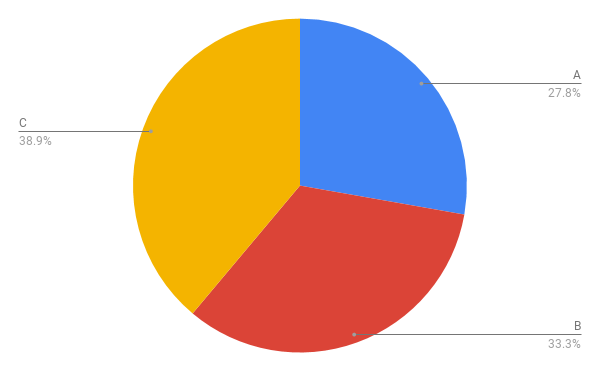
\includegraphics[width=0.5\textwidth]{reproduction_chart.png}
	\caption{The roulette wheel from my proportional selection example}
	\label{fig:roulette_wheel}
	\end{center}
\end{figure}
Tournament selection could be translated in the following way. Have an empty list which will contain an ordered list of agents. In a loop (until the population is of size 1): select two agents from the population, remove the lowest fitness one and insert it into the list. After the loop insert the last agent into the top of the list. The top of the list always contains the highest fitness agent. Using the same population of agents in the proportional selection algorithm we can give an example of this in table~\ref{tab:tournament_selection}.
\begin{framed}
	\begin{center}
		\begin{tabular}{c|c|c|c}
		Set & Test & Put in List & List\\
		\hline
		${A_1, A_2, B_1, B_2, B_3, B_4, C_1}$ & $(A_1, B_3)$ & $A_1$ & ${A_1}$ \\
		${A_2, B_2, B_3, B_4, C_1}$ & $(B_1, C_1)$ & $B_1$ & ${A_1, B_1}$\\
		${B_2, B_3, B_4, C_1}$ & $(A_2, C_1)$ & $A_2$ & ${A_1, B_1, A_2}$\\
		${B_2, B_3, C_1}$ & $(B_4, C_1)$ & $B_4$ & ${A_1, B_1, A_2, B_4}$\\
		${B_3, C_1}$ & $(B_2, B_3)$ & $B_2$ & ${A_1, B_1, A_2, B_4, B_2}$\\
		${B_3}$ & $(B_3, C_1)$ & $C_1$ & ${A_1, B_1, A_2, B_4, B_2, C_1}$\\
		$\emptyset$	& & $B_3$ & ${A_1, B_1, A_2, B_4, B_2, C_1, B_3}$
		\end{tabular}
		\captionof{table}{The payoff for my indirect reciprocity model}
		\label{tab:tournament_selection}
	\end{center}	
\end{framed}
Fitness proportionate selection seems to translate best to my system as there is an obvious and simple way to select each agents strategy for the new generation using the roulette wheel, unlike the tournament selection process which requires the crossover step. The crossover step requires a chromosome represented as a bit array to produce an offspring from two parents. This is analogous to sexual reproduction, but not the building of new agents.\par
Lipowski \textit{et al.}~\cite{lipowski2012roulette} presented an efficient version of roulette wheel selection using stochastic acceptance rather than the searching method used by Francq~\cite{genetic_algorithms}. The stochastic acceptance algorithm works like this: select randomly one of the individuals from the last generations population, with fitness of the individual as $w_i$ and $w_{max}$ the maximal fitness of the generation use the probability $w_i / w_{max}$ to select whether or not to use this agents strategy for a new generation agent, if not repeat. Lipowski \textit{et al.} proved mathematically that the probability distribution of this method and general roulette wheel selection are the same, and that the stochastic acceptance algorithm is more efficient as well.\par
Due to these factors I have decided to use the roulette wheel-selection via stochastic acceptance algorithm proposed by Lipowski \textit{et al.} with a user-selectable chance of random mutation for each new agent.

\subsection{Agents}
Franklin and Graesser~\cite{franklin1996agent} stipulated that to describe an agent one must describe five aspects: the environment the agent resides in, the agent's sensing capabilities, the possible actions the agent can take, the drives or primative motivators for an agents actions and the action selection architecture for the agent. The first three I have described clearly in the previous subsections in this section, the drive of each agent I have alluded to throughout my literary review and the previous subsections of this section - I will be further describing this in subsections~\ref{subs:strat} and~\ref{subs:trustm}. In this subsection I will describe the action selection architecture my agents use.\par
I have previously briefly discussed the internal state described by Russell and Norvig~\cite{russell2016artificial}, and the beliefs of the BDI model first presented by Bratman~\cite{bratman1987intention} which I plan to emulate to store image scores and beliefs on the standing of other agents. Events in the BDI model may cause an agent to update beliefs, trigger plans or modify goals~\cite{kostas_deductive}. My agents will use percepts as events to update their beliefs.\par
How an agent uses the percepts to update their beliefs is down to the trust model of the agent which I will describe in subsection~\ref{subs:trustm}. From an architectural standpoint I will be using the 'multi-valued fluent cached event calculus' (MVFCEC)~\cite{mvfcec} to reason about events and how they effect beliefs. The essence of the event calculus is that events occur at specific timepoints, these events initiate and terminate periods of time for which a fluent holds. For example at time $t1$ event $e1$ occurs, fluent $f$ did not hold prior to $e1$, but $e1$ initiated it and as such it holds after $t1$. A second event $e2$ then occurs at timepoint $t2$ where $t2>t1$, this event terminates $f$. Following this event $f$ no longer holds, but $f$ still holds in between $t1$ and $t2$.\par
The beliefs in my system will be the combination of the value and the fluent of multi-valued fluents~\cite{artikis2009specifying}. For example the fluent $standing(agent1, agent2, t)=value$ is the belief of $agent1$ on the standing of $agent2$ and timepoint $t$, in this fluent the value can either be good or bad. MVFCEC is an efficient version of the event calculus that uses multi-valued fluents, and was developed by Kostas Stathis~\cite{mvfcec}.\par
In Yoav Shohams's Agent0 language~\cite{shoham1991agent0} there are two mental categories: beliefs and commitments. He defines beliefs as a fact that is thought to be true by an agent at a specific time about a specific time, as such I have already described my systems version of beliefs. Commitments are given by Shoham as a commitment to act. An agent is constrained in making a commitment by the agents capabilities i.e. an agent can only commit to an action if they believe they are capable of it.\par 
These three concepts - beliefs, commitments and capabilities - are included in my agent design, in which an agent makes a commitment to action, based upon it's beliefs about the environment and other agents, and it's beliefs on it's own capabilities. This way I can constrain an agent to only be capable of cooperating or defecting when the agent is a donor in an interaction.\par
Russell and Norvig~\cite{russell2016artificial} describe a number of agent architectures including the model-based reflex agent (illustrated in figure~\ref{fig:model_reflex}). My agents follow this architecture. The state is the beliefs system I have described, which is revised by percepts from the environment. The condition-action rules are constrained by the agents capabilities and what the agent decides to do is a commitment.\par
The final aspect to describe is the condition-action rules themselves. An agent is associated to a strategy, this strategy defines the condition-action rules the agent uses. The rules themselves are written in a teleo-reactive~\cite{nilsson1993teleo} structure. This teleo-reactive structure was promoted by Nilsson as a decision making component for agents in dynamic environments. Although my environment is static, the structure a teleo-reactive program takes is ideal for decision making based on beliefs.\par
This structure is a set of conditions that imply actions, as illustrated in table~\ref{tab:trrules} in which $K_i$ are conditions and $a_i$ are actions. The sequence is interpretted from the top down, in which the first condition that matches is then committed to by the agent. At the decision stage of each timepoint every agent makes a decision based by searching through the sequence of teleo-reactive rules their assigned strategy has. There is a default action at the very end of every strategies teleo-reactive program, which is the idle action.\par
The conditions $K_i$ are a mix of the agents beliefs and capability beliefs. For example an agent only believes they are capable of a donor action with another agent if they are the donor and the other agent is a recipient in a donor-recipient pair, say this agent was using the `Cooperator' strategy, and they believed themselves capable of this then the agent will commit to a cooperation donor action towards the other agent. The commitment to this action was made as it was the first condition set that matched the situation, coming before the default idle action in the teleo-reactive sequence and other possible condition sets.\par
The teleo-reactive programming of the system is a theory of how to act based on logical rules and the beliefs system acts as a logical database to describe the state of the world. A deductive reasoning agent encodes a theory on how to act in a given situation~\cite{kostas_deductive} and as such my agents are deductive reasoning agents.
\begin{framed}
	\begin{center}
		\begin{tabular}{c}
		$K_1 \rightarrow a_1$\\
		$K_2 \rightarrow a_2$\\
		$\cdot \cdot \cdot$\\
		$K_m \rightarrow a_m$
		\end{tabular}
		\captionof{table}{A teleo-reactive program}
		\label{tab:trrules}
	\end{center}	
\end{framed}
\begin{figure}
	\begin{center}
	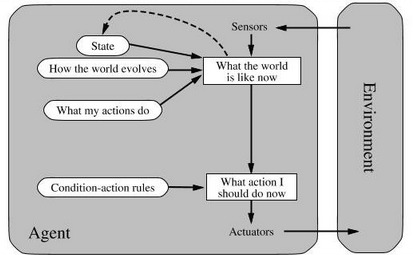
\includegraphics[width=0.5\textwidth]{RuNorv.png}
	\caption{A model-based reflex agent from Russell and Norvig~\cite{russell2016artificial}.}
	\label{fig:model_reflex}
	\end{center}
\end{figure}


\subsection{Strategies}
\label{subs:strat}
In my system an agent is associated with a strategy. This strategy describes how an agent will act in any given situation it comes across. A strategy is encoded in my system using a teleo-reactive sequence. Each strategy that is programmed has one or multiple drive in it's design. For example, the standing strategy is driven to facilitate the evolution cooperation in a system by cooperating with those it sees as valuable in a society and punishing those who are uncooperative to valuable members of a society, the strategy is also driven to improve it's own standing in the society by acting cooperatively and in turn improve it's own fitness due to the mechanism of indirect reciprocity~\cite{imagevsstanding}.\par
The drive of the image scoring discriminator is the same. Another strategy that uses it's own image score as a decision basis is more clearly driven by the desire to improve it's own fitness. This strategy works out when it is important to improve it's reputation in a community by cooperating and when it is safe to defect without reducing it's own image score to levels in which it won't receive cooperation from others. This prevents agents using the strategy from committing to costly cooperations, when it is safe to defect. Then there is the two naive strategies: defector and cooperator. A defector always defects when given the opportunity and a cooperator always cooperates.\par
So far I have only described strategy component of when agents are acting as donors, but statistically an agent is only likely to be a donor $m/n$ times when $m$ is the number of timepoints in a generation and $n$ is the number of agents in the generation. Furthermore, a strategy is by definition a description of how to act under any circumstances. Agents the majority of the time will not be acting as a donor, and thus strategies described above must be associated with components that describe how to act when the agent is not a donor.\par
The action options agents have is to either be idle or to gossip. A very simple strategy component for this is the `lazy' strategy, in which an agent is always idle when not a donor. One of Baumeister \textit{et al.}'s functions of gossip is to strengthen bonds between the recipient and the gossiper. This drive is the drive behind another strategy: `promote self'. This strategy promotes an agent by gossiping positively about themself to other agents. The recipient of this self-promotion could be either directed towards specific agents, or naively spread at random to known agents.\par
A defector could also be seen as having the drive to disrupt a system for it's own ends: to channel cooperation towards itself and to avoid costly cooperation itself. The defector strategy can use the `promote self' strategy when it is not a donor to deceive agents into acting cooperatively towards it, despite the defectors uncooperative actions. This would only affect agents that trust gossip from the defector, but some agent strategies may be naive enough to trust it (more on this in subsection~\ref{subs:trustm}).\par
Another method of deception and manipulation an defector can use is the `spread negative' strategy component, which spreads negative information about other agents among the system. This simulates what might be known as `fake news', which is a highly discussed topic at the moment and allows an agent to manipulate who cooperates with whom. It has a strong effect on the standing strategy. Take 3 agents: $a$, $b$ and $c$. $a$ is a defector using the `spread negative' strategy component, $b$ is using the standing strategy and trusts $a$'s gossip. $a$ gossips to $b$ negatively about $c$, consequently $c$ has a bad standing according to $b$. $a$ is now able to defect against $c$ without reducing it's standing with $b$ and decreasing it's chance of receiving cooperation from that agent.\par
Another case in which manipulation can occur within my system, is accidental manipulation by naive agents. This is evident in the cooperator strategy being able to use the `spread positive' strategy component. This component aimlessly spreads positive gossip about other agents. With this strategy I wish to examine the effect of naive strategies on the evolution of cooperation.\par
The last two strategy components for when the agent is not a donor I will discuss are: `spread accurate positive' and `spread accurate negative'. These two strategy components spread what they believe is accurate information about agents in the system to those they trust. This requires an agent to have beliefs on the reputation of an agent in the system, unlike naive agents such as cooperator, defector and random. Agents that using image scores and the standing strategy have the means to do this.\par
For example, image scoring agents using the `spread accurate negative' strategy component that have the discriminator value of $k$ will spread negative gossip about those with a value of less than $k$ to other agents will a value of greater than or equal to $k$. Another example being standing strategy agents using the `spread accurate positive' will spread positive gossip about agents they believe to have a good standing to others which they believe to have a good standing.\par
All the strategy components I have mentioned above are included in my system and associated correctly to make full strategies (all strategies in the system are listed in the appendix in section~\ref{appendix:strats}). It is also worth mentioning that reinforcement strategies could be effective in this system - as they have been in the iterated prisoner's dilemma~\cite{harper2017reinforcement}. Howerver, it would be interesting to see how delayed rewards and deception and manipulation affect a reinforcement learning model.

\subsection{Trust Models}
\label{subs:trustm}
So now we have strategies for how to act given circumstances and the agents beliefs, but how do these agents form those beliefs? I have described the use of percepts as events for the MVFCEC, but how an agent interprets these percepts to form beliefs is down to the agents trust model. Certain trust models are associated with certain strategies in the system.\par
Each trust model has a method for handling any percept that is important to the updating of the agents beliefs. Cooperators, defectors and the random strategy do not require trust models as they have no belief system. The more interesting strategies that use image scores and the standing strategy do, however, require trust models.\\
I shall go through these on a percept by percept basis. First off let us consider the direct observation of a defection. In an image scorer using any trust model, the image score of the defecting player is reduced by 1. In the standing strategy the defecting player is reduced to a bad standing if the recipient is considered to have a good standing by the observing agent, if the recipient has a bad standing then no update is made on the observers beliefs.\par
Then let us consider being a recipient of a defection. This is the same interpretation of the event as for a direct observation of a defection, except for in the `personal grievance' trust model for image scorers in which the image score is reduced by two rather than one.\par
There is a mirror for this in direct observation of a cooperation by an image scorer in which the image score of the donor increases by one. When using the `personal grievance' trust model, if receiving a cooperation an agent increases the image score of the donor by two. Interpretation of cooperation differs from interpretation of defection for the standing strategy, which when observing or being the recipient of a cooperation sets the standing of the donor to a good standing.\par
Further to interpretation of interaction event percepts there is also intepretation of gossip to consider. I have split this into three trust models: 'naive trusting', 'trusting' and 'distrusting'. `Distrusting' is the easiest model to describe, this model abjectly ignores any gossip it receives no matter who gossiped or who it is about. At the other end of the spectrum the `naive trusting' model trusts any gossip it receives, no matter whom it is from or about.\par
For an image scorer using the `naive trusting' model, positive gossip increases the image score of the agent which the gossip is about by one, and negative gossip decreases the image score of the agent the gossip is about by 1. For an agent using the standing strategy and the `naive trusting' model, positive gossip changes the standing of the agent the gossip is about to bad and negative gossip changes it to good.\par
The more interesting trust model out of the three is `trusting'. This model is less black and white. A `trusting' image scorer will only change its beliefs if the gossip comes from a source which the agent `trusts' i.e. the gossiper has an image score of greater than the value $k$ which the image scorer has been set up with. It is the same for standing strategy agents, except which the agents they `trust' are those with a good standing.\par
The list of strategies in the appendix (section~\ref{appendix:strats}) also includes all the trust models each strategy is associatable to, which have each been outlined in detail here. 

\subsection{Summary}
\noindent
In summary I have discussed the operation of the environment including:
\begin{itemize}
	\item how communities function with a reproduction mechanism between generations and fitness scoring system
	\item the discrete timepoints within the generations in which the synchronised perceive-decide-execute cycle occurs
	\item the percepts and actions (including gossip) that can be produced in the environment
	\item the properties of the environment
\end{itemize} 
Further to this, I have described the theoretical agents in my system including:
\begin{itemize}
	\item agent beliefs, commitments and capabilities systems
	\item agent architecture
	\item teleo-reactive action selection
	\item strategies
	\item trust models
\end{itemize}
\par
By design the agents in the theoretical framework I have described satisfies the four properties of Wooldridge and Jennings'~\cite{wooldridge_jennings_1995} weak notion of agency: autonomy, social ability, reactivity and proactivity. Agents use their trust models, beliefs and teleo-reactive sequences to decide on what actions to take, making them autonomous. Agents are capable of using SAGL to interact with other agents via gossip actions. Using teleo-reactive sequence a strategy is able to react to percepts, such as perceiving that they are a donor in a donor-recipient pair and acting accordingly. My architecture also allows agents to be proactive by gossiping at times which they are not a donor, promoting themselves proactively or spreading accurate or inaccurate information.\par
The next phase is to implement this framework in a multi-agent system which I will describe in the next section of this chapter.

\section{Implementation}
\textcolor{red}{Relate to agents systems.\\
Making it distributable.\\
Objectives 5 and 6\\
AMAAS.\\
Logic framework.\\
Include software engineering, algorithmic work and development processes. In their own sections.\\
Body and mind separate.}\par



\subsection{Agent Mind as a Service}
\subsection{Environment}
\subsection{Web Application and Interface}
\subsection{Conclusion}

\section{Technical Preparation}
\textcolor{red}{Learning flask etc.}

\section{Design}

\subsection{Agent Mind as a Service}
\subsection{Environment}
\subsection{Web Application and Interface}

\section{Development}

\subsection{Agent Mind as a Service}
\subsection{Environment}
\subsection{Web Application and Interface}

\section{Testing}

\subsection{Agents Service Testing}
\subsection{Environment Testing}
\subsection{Web Application Testing}

\section{Software Engineering}

\section{Documentation}
\textcolor{red}{Software documentation, user guide.}

\chapter{Experiment Evaluation}
\section{Introduction}
\textcolor{red}{What experiments will I be doing, why?\\
Look at the summary of my background for what to experiment with.\\
Factors that could effect cooperation:
\begin{itemize}
	\item Number of generations
	\item Strategy
	\item Trust Model
	\item Whether a player knows the reputation of another player (generation size, generation length (2m/n~\cite{evol_indirect_image}), onlooker number and social activeness)
	\item Positivity of gossip vs Accuracy of gossip
	\item Deception and manipulation (image vs standing)
	\item Sommerfeld's 3 properties
\end{itemize}
Control variables:
\begin{itemize}
	\item Number of generations
	\item Mutation chance
	\item How many experiment repetitions? ( due to non-determinicity of the game)
\end{itemize}}


\section{Experiment 1}
\textcolor{red}{Variable setting, controls etc.\\
Evaluation}

\section{Experiment 2}

\section{Experiment n}

\section{Discussion}
\textcolor{red}{Evaluation and discussion on the experiments\\
Successful?\\
Opportunity for extra work?\\
Focus on experiments}

\chapter{Critical Analysis and Discussion}
\textcolor{red}{Project achievements\\
Reflection on project process (difficulties, success, failure)\\
Successful?\\
Future enhancements\\
Focus on project\\
Compare to deliverables at beginning.}

\chapter{Conclusions}
\textcolor{red}{Mechanism has to work with and without re-meeting.\\
Mechanism has to encourage cooperation between unknown entities.\\
Opportunity for extra work? Further exploration of network reciprocity as outline in background and background summary. Extend indirect reciprcoty so individuals can choose who they wish to interact with. Symbolic reinforcement learning strategies~\cite{harper2017reinforcement}.\\
Move closer to using an agent model such as BDI?\\
Using the GAIA methodology for development?~\cite{wooldridge2000gaia}.\\
Reaching agreements\\
Use an AOP language (GOAL or SARL?)}



%%%% ADD YOUR BIBLIOGRAPHY HERE
\newpage
\bibliography{../../refs.bib}{}
\bibliographystyle{plain}
\addcontentsline{toc}{chapter}{Bibliography}
\label{endpage}

\chapter{Professional Issues}
\textcolor{red}{Replacement of people in jobs?\\
AI issues and risks?\\
Relate to project\\
Moral philosophy of agent societies\\
Refer to last chapter of russell and norvig}

\chapter{Appendix}
\label{appendix}
\textcolor{red}{Describe the contents of my appendix.}
\section{Strategies}
\label{appendix:strats}
\textcolor{red}{include list of strategy components and trust models, all associated together}.

%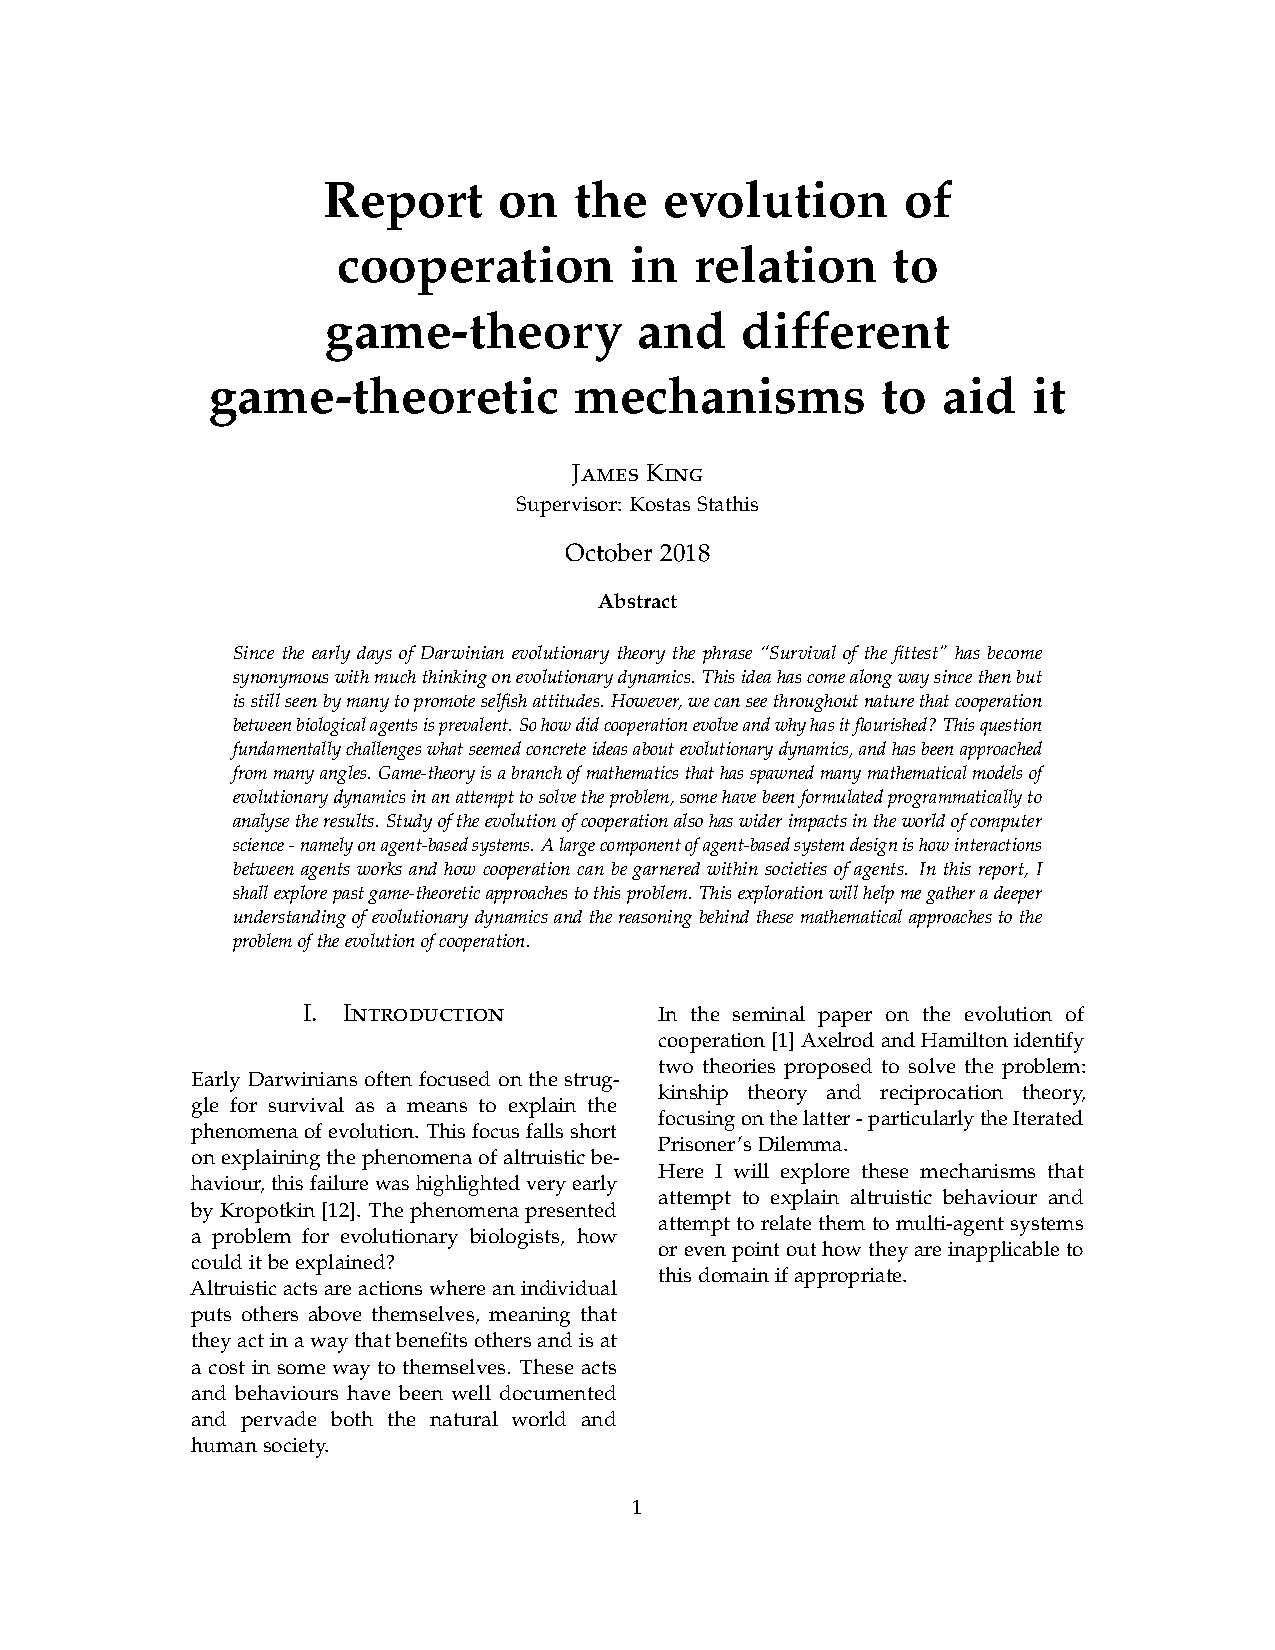
\includepdf[pages=-]{../../EvolCoop/EvolCoopReport.pdf}

%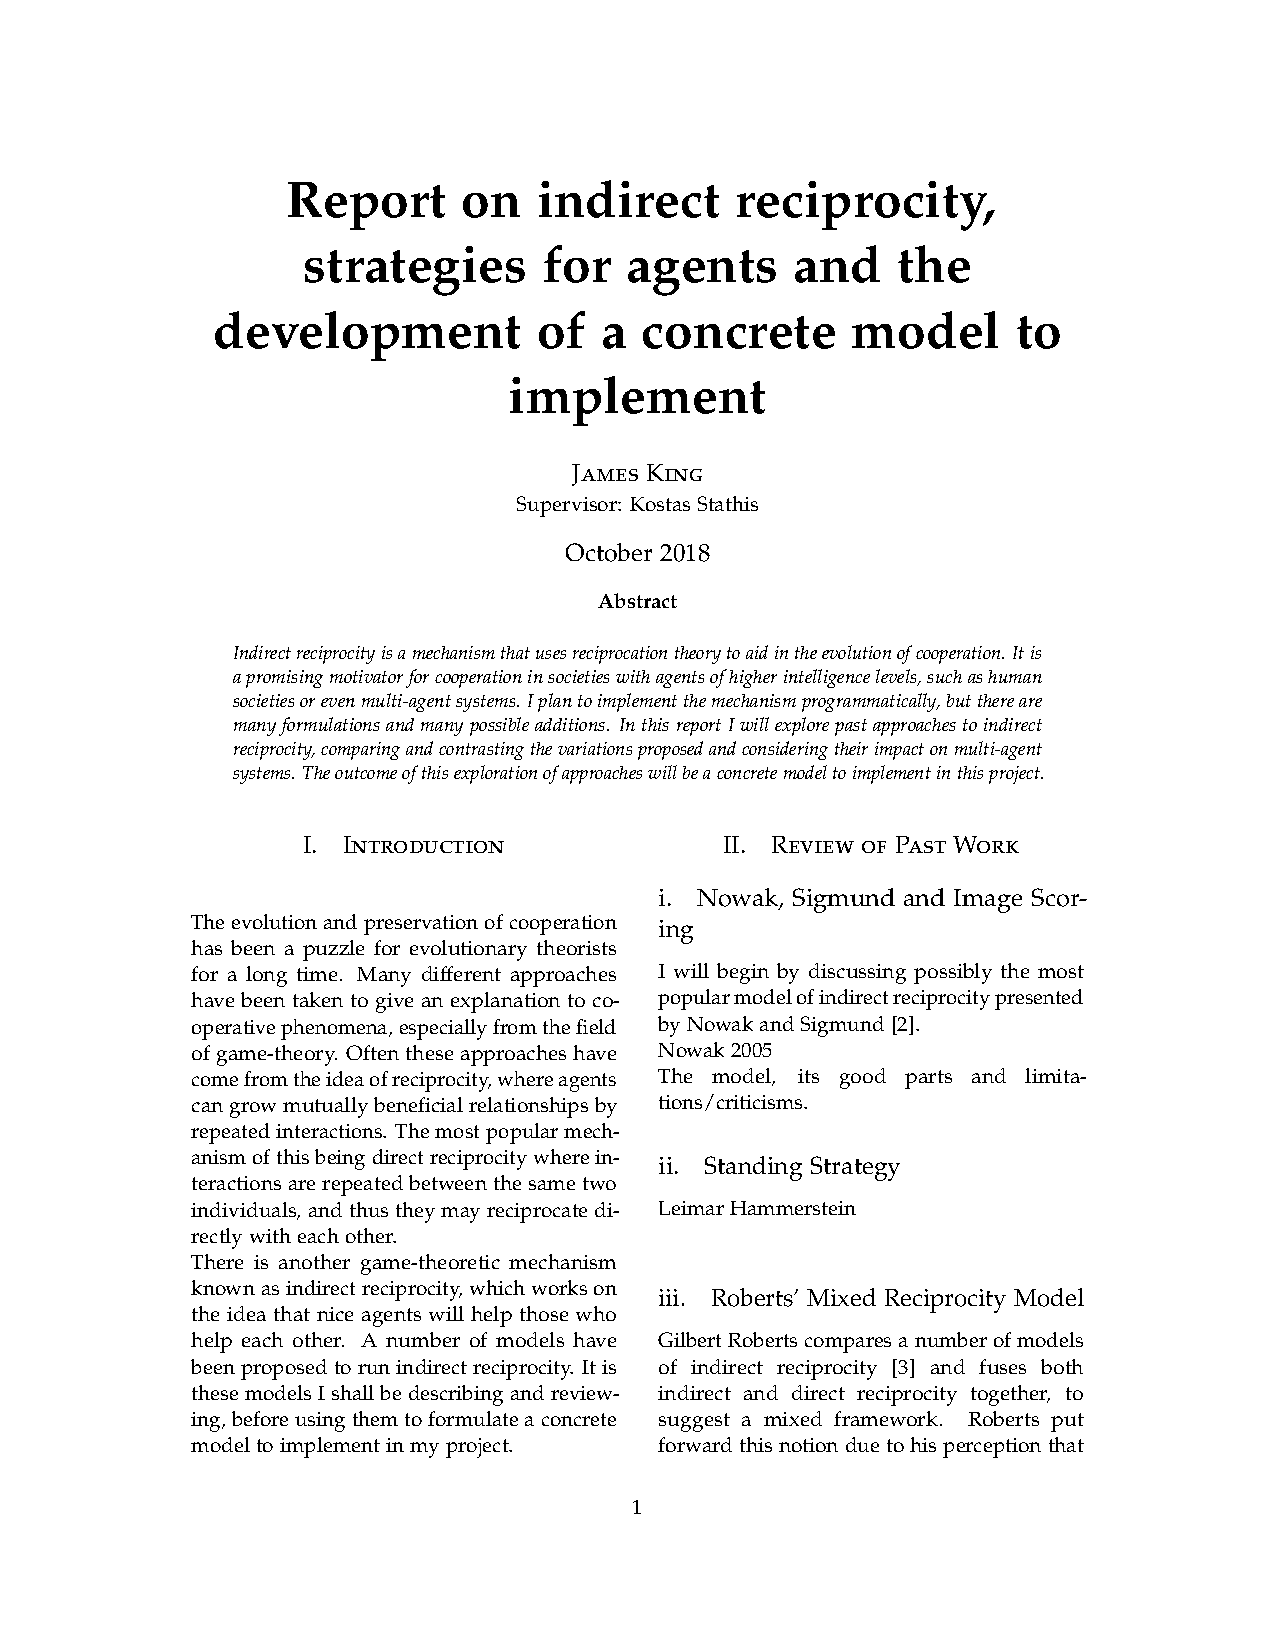
\includepdf[pages=-]{../../IndirRec/IndirRec.pdf}

%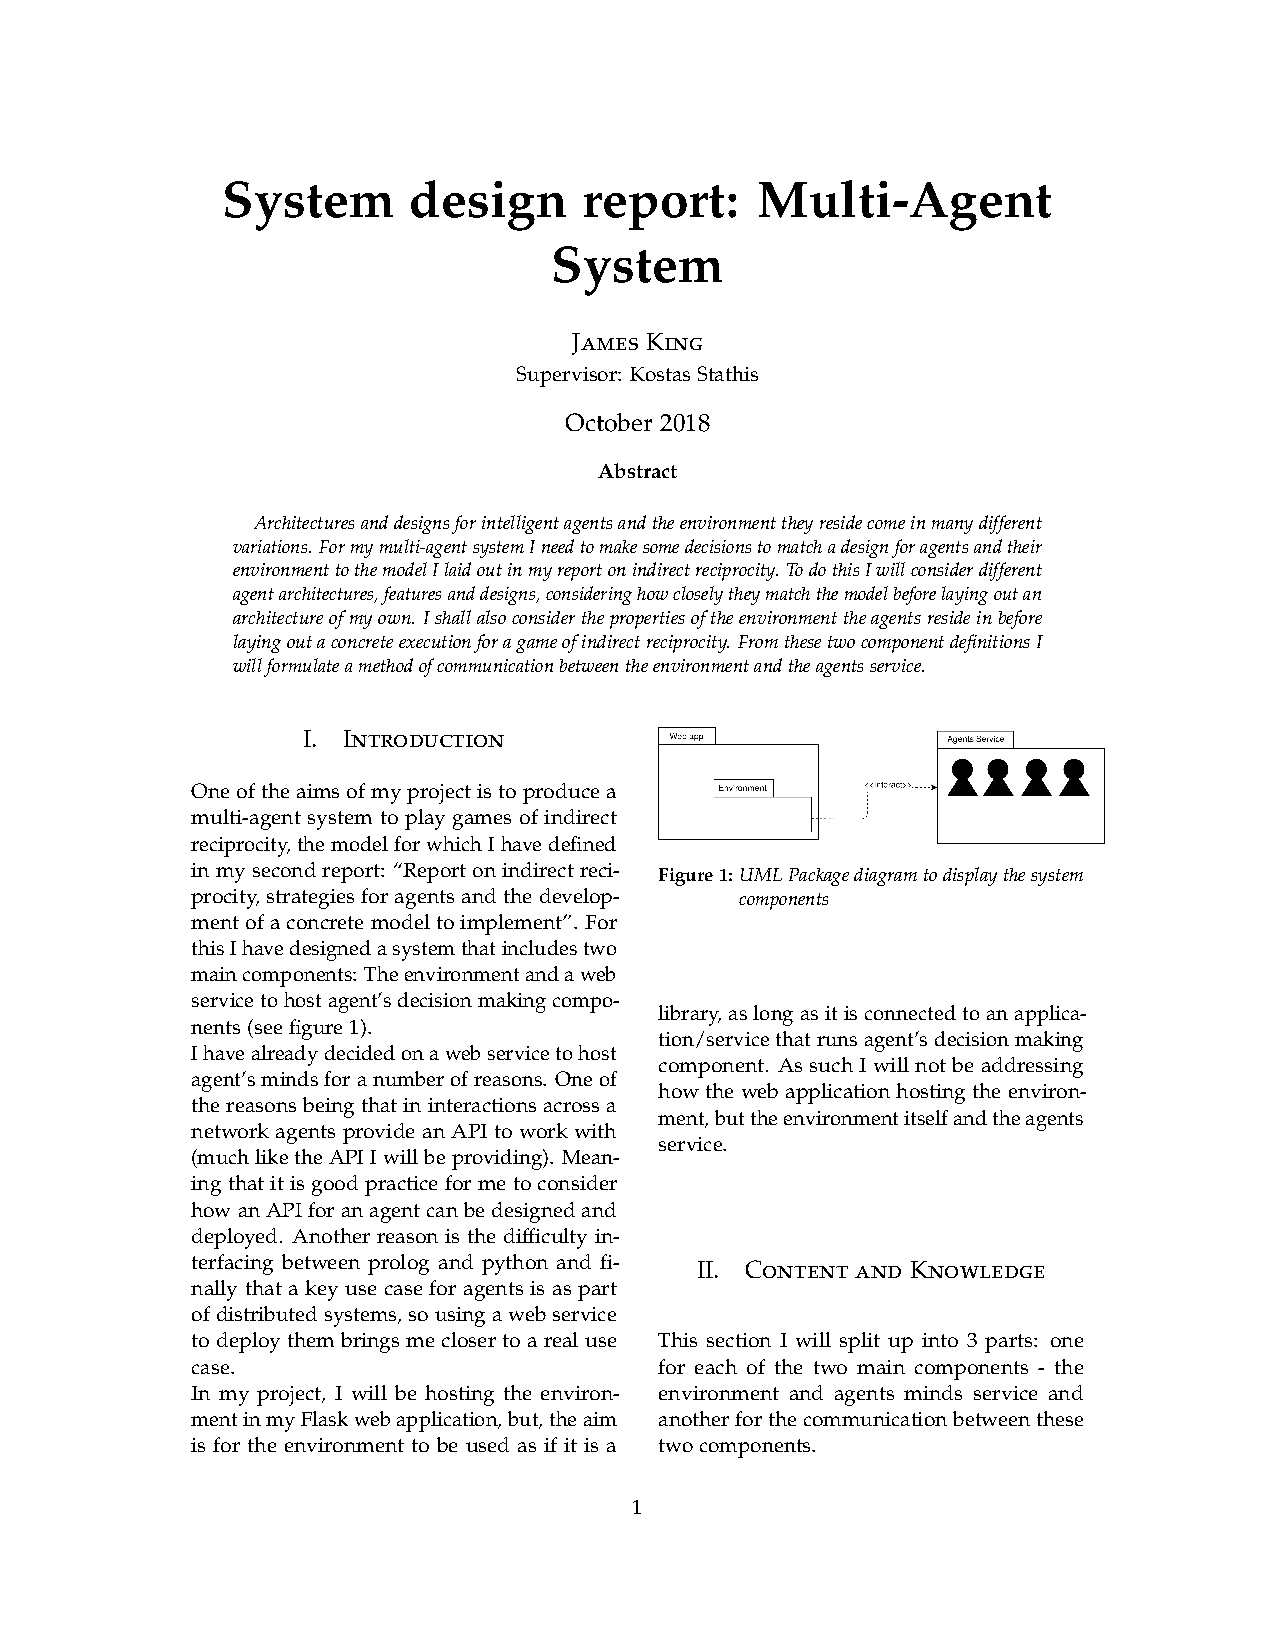
\includepdf[pages=-]{../../SysDesign/SysDesign.pdf}

%\begin{figure}
%	
\includepdf[pages=-,link=true,linkname=web_app_testing]{../../TestingStrategy/TestingStrategy.pdf}
%	\caption{\label{appendix:web_app_testing}}
	
%\end{figure}


\end{document}

\end{article}
